%%%%%%%%%%%%%%%%%%%%%%%%%%%%%%%%%%%%%%%%%%%%%%%%%%%
%% LaTeX book template                           %%
%% Author:  Amber Jain (http://amberj.devio.us/) %%
%% License: ISC license                          %%
%%%%%%%%%%%%%%%%%%%%%%%%%%%%%%%%%%%%%%%%%%%%%%%%%%%
\documentclass[12pt,french,twoside,openright]{book}

%\documentclass[a4paper,11pt]{book}
\usepackage[T1]{fontenc}
\usepackage[utf8]{inputenc}
\usepackage{lmodern}
%%%%%%%%%%%%%%%%%%%%%%%%%%%%%%%%%%%%%%%%%%%%%%%%%%%%%%%%%
% Source: http://en.wikibooks.org/wiki/LaTeX/Hyperlinks %
%%%%%%%%%%%%%%%%%%%%%%%%%%%%%%%%%%%%%%%%%%%%%%%%%%%%%%%%%
\usepackage{hyperref}
\usepackage{graphicx}
\usepackage[francais]{babel}
\usepackage{pdfpages}
\usepackage{amsmath}
\usepackage{amssymb}
\usepackage{a4}
\usepackage{indentfirst}
\usepackage{fancyhdr}
\usepackage{varioref}
\usepackage{makeidx}


%%%%%%%%%%%%%%%%%%%%%%%%%%%%%%%%%%%%%%%%%%%%%%%%%%%%%%%%%%%%%%%%%%%%%%%%%%%%%%
%%%%%%%%%%%%%%%%%%%%%%%%%%%%%%%%%%%%%%%%%%%%%%%%%%%%%%%%%%%%%%%%%%%%%%%%%%%%%%

\pagestyle{fancy}

\addtolength{\headwidth}{\marginparsep}
\addtolength{\headwidth}{\marginparwidth}
\renewcommand{\chaptermark}[1]{\markboth{#1}{}}
\renewcommand{\sectionmark}[1]{\markright{\thesection\ #1}}
\fancyhf{}
\fancyhead[LE,RO]{\bfseries\thepage}
\fancyhead[LO]{\bfseries\rightmark}
\fancyhead[RE]{\bfseries\leftmark}
\fancypagestyle{plain}{
\fancyhead{} % get rid of headers
\renewcommand{\headrulewidth}{0pt} % and the line
}

\voffset -1.04cm
\textheight 25cm
\hoffset -1in
\evensidemargin 2.5cm
\oddsidemargin 2.5cm
\textwidth 16cm

%%%%%%%%%%%%%%%%%%%%%%%%%%%%%%%%%%%%%%%%%%%%%%%%%%%%%%%%%%%%%%%%%%%%%%%%%%%%%%
%%%%%%%%%%%%%%%%%%%%%%%%%%%%%%%%%%%%%%%%%%%%%%%%%%%%%%%%%%%%%%%%%%%%%%%%%%%%%%

%\textwidth16cm
%\textheight23cm
%\oddsidemargin0,5cm
%\evensidemargin0,5cm
\topmargin-1cm
%\parskip0,5cm
%\parindent0cm



%%%%%%%%%%%%%%%%%%%%%%%%%%%%%%%%%%%%%%%%%%%%%%%%%%%%%%%%%%%%%%%%%%%%%%%%%%%%%%%%
% 'dedication' environment: To add a dedication paragraph at the start of book %
% Source: http://www.tug.org/pipermail/texhax/2010-June/015184.html            %
%%%%%%%%%%%%%%%%%%%%%%%%%%%%%%%%%%%%%%%%%%%%%%%%%%%%%%%%%%%%%%%%%%%%%%%%%%%%%%%%
\newenvironment{dedication}
{
   \cleardoublepage
   \thispagestyle{empty}
   \vspace*{\stretch{1}}
   \hfill\begin{minipage}[t]{0.66\textwidth}
   \raggedright
}
{
   \end{minipage}
   \vspace*{\stretch{3}}
   \clearpage
}

%%%%%%%%%%%%%%%%%%%%%%%%%%%%%%%%%%%%%%%%%%%%%%%%
% Chapter quote at the start of chapter        %
% Source: http://tex.stackexchange.com/a/53380 %
%%%%%%%%%%%%%%%%%%%%%%%%%%%%%%%%%%%%%%%%%%%%%%%%
\makeatletter
\renewcommand{\@chapapp}{}% Not necessary...
\newenvironment{chapquote}[2][2em]
  {\setlength{\@tempdima}{#1}%
   \def\chapquote@author{#2}%
   \parshape 1 \@tempdima \dimexpr\textwidth-2\@tempdima\relax%
   \itshape}
  {\par\normalfont\hfill--\ \chapquote@author\hspace*{\@tempdima}\par\bigskip}
\makeatother


% Babel ``Sommaire'' à la place de ``table des matières''
\renewcommand{\contentsname}{Sommaire}


%%%%%%%%%%%%%%%%%%%%%%%%%%%%%%%%%%%%%%%%%%%%%%%%%%%
% First page of book which contains 'stuff' like: %
%  - Book title, subtitle                         %
%  - Book author name                             %
%%%%%%%%%%%%%%%%%%%%%%%%%%%%%%%%%%%%%%%%%%%%%%%%%%%

% Book's title and subtitle
\title{\Huge \textbf{Apprentissage dans les architectures cognitives}   \\ \huge contributions pour l'informatique et les neurosciences}
% Author
\author{\textsc{Emmanuel Daucé}}%\thanks{\url{www.example.com}}}


\begin{document}

\frontmatter
\maketitle

%%%%%%%%%%%%%%%%%%%%%%%%%%%%%%%%%%%%%%%%%%%%%%%%%%%%%%%%%%%%%%%
% Add a dedication paragraph to dedicate your book to someone %
%%%%%%%%%%%%%%%%%%%%%%%%%%%%%%%%%%%%%%%%%%%%%%%%%%%%%%%%%%%%%%%
\begin{dedication}
Dedicated to Calvin and Hobbes.
\end{dedication}

%%%%%%%%%%%%%%%%%%%%%%%%%%%%%%%%%%%%%%%%%%%%%%%%%%%%%%%%%%%%%%%%%%%%%%%%
% Auto-generated table of contents, list of figures and list of tables %
%%%%%%%%%%%%%%%%%%%%%%%%%%%%%%%%%%%%%%%%%%%%%%%%%%%%%%%%%%%%%%%%%%%%%%%%
\tableofcontents
\listoffigures
\listoftables

\mainmatter

\section*{Remerciements}
\begin{itemize}
\item A special word of thanks goes to Professor Don Knuth\footnote{\url{http://www-cs-faculty.stanford.edu/~uno/}} (for \TeX{}) and Leslie Lamport\footnote{\url{http://www.lamport.org/}} (for \LaTeX{}).
\item I'll also like to thank Gummi\footnote{\url{http://gummi.midnightcoding.org/}} developers and LaTeXila\footnote{\url{http://projects.gnome.org/latexila/}} development team for their awesome \LaTeX{} editors.
\item I'm deeply indebted my parents, colleagues and friends for their support and encouragement.
\end{itemize}
\mbox{}\\
%\mbox{}\\
\noindent Amber Jain \\
\noindent \url{http://amberj.devio.us/}

%%%%%%%%%%%%%%%%
% NEW CHAPTER! %
%%%%%%%%%%%%%%%%


%%%%%%%%%%%%%%%%%%%%%%%%%%%%%%%%%%%%%%%%%%%%%%%%%%%%%%%%%%%%%%%%%%%%%%%%%%%%%%%%%%%%%%%%%%%%%%%%%%%%%%%%%%%%%%%%%%%
%%%%%%%%%%%%%%%%%%%%%%%%%%%%%%%%%%%%%%%%%%%%%%%%%%%%%%%%%%%%%%%%%%%%%%%%%%%%%%%%%%%%%%%%%%%%%%%%%%%%%%%%%%%%%%%%%%%
%%%%%%%%%%%%%%%%%%%%%%%%%%%%%%%%%%%%%%%%%%%%%%%%%%%%%%%%%%%%%%%%%%%%%%%%%%%%%%%%%%%%%%%%%%%%%%%%%%%%%%%%%%%%%%%%%%%
%%%%%%%%%%%%%%%%%%%%%%%%%%%%%%%%%%%%%%%%%%%%%%%%%%%%%%%%%%%%%%%%%%%%%%%%%%%%%%%%%%%%%%%%%%%%%%%%%%%%%%%%%%%%%%%%%%%
%%%%%%%%%%%%%%%%%%%%%%%%%%%%%%%%%%%%%%%%%%%%%%%%%%%%%%%%%%%%%%%%%%%%%%%%%%%%%%%%%%%%%%%%%%%%%%%%%%%%%%%%%%%%%%%%%%%
%%%%%%%%%%%%%%%%%%%%%%%%%%%%%%%%%%%%%%%%%%%%%%%%%%%%%%%%%%%%%%%%%%%%%%%%%%%%%%%%%%%%%%%%%%%%%%%%%%%%%%%%%%%%%%%%%%%


\chapter{Introduction}


%%%%%%%%%%%%%%%%%%%%%%%%%%%%%%%%%%%%%%%%%%%%%%%%%%%%%%%%%%%%%%%%%%%%%%%%%%%%%%%%%%%%%%%%%%%%%%%%%%%%%%%%%%%%%%%%%%%
%%%%%%%%%%%%%%%%%%%%%%%%%%%%%%%%%%%%%%%%%%%%%%%%%%%%%%%%%%%%%%%%%%%%%%%%%%%%%%%%%%%%%%%%%%%%%%%%%%%%%%%%%%%%%%%%%%%
%%%%%%%%%%%%%%%%%%%%%%%%%%%%%%%%%%%%%%%%%%%%%%%%%%%%%%%%%%%%%%%%%%%%%%%%%%%%%%%%%%%%%%%%%%%%%%%%%%%%%%%%%%%%%%%%%%%
%%%%%%%%%%%%%%%%%%%%%%%%%%%%%%%%%%%%%%%%%%%%%%%%%%%%%%%%%%%%%%%%%%%%%%%%%%%%%%%%%%%%%%%%%%%%%%%%%%%%%%%%%%%%%%%%%%%
%%%%%%%%%%%%%%%%%%%%%%%%%%%%%%%%%%%%%%%%%%%%%%%%%%%%%%%%%%%%%%%%%%%%%%%%%%%%%%%%%%%%%%%%%%%%%%%%%%%%%%%%%%%%%%%%%%%
%%%%%%%%%%%%%%%%%%%%%%%%%%%%%%%%%%%%%%%%%%%%%%%%%%%%%%%%%%%%%%%%%%%%%%%%%%%%%%%%%%%%%%%%%%%%%%%%%%%%%%%%%%%%%%%%%%%



\begin{chapquote}{Author's name, \textit{Source of this quote}}
``This is a quote and I don't know who said this.''
\end{chapquote}

% le modèle de Hopfield
% Qu'est-ce que le chaos?

% Qu'est-ce qu'un système apprenant



% Architectures de contrôle. Point de vue de la robotique. Automates embarqués. 

Quelle est la question?


% Philo
Créer du neuf à partir de rien.
Qu'est-ce que la nouveauté?
D'où vient l'information?

Potentialité et émergence. Notion d'historique. Constructivisme.
% Importance de l'activité intrinsèque
% Activité centrale flutuante, émergence, historique
% couplage sans fonction (corps sans organe)
% triptique : corps- société- organe (à différents niveaux) - organisme = société des organes
% analogie eonomique : composants - emploi - produit (composé)

% Ce que j'ai fait, quelles sont mes questions?

Les enjeux :

- Substrat apprenant (universel). 

- Aller au delà des modèles actuels de l'apprentissage (essentiellement behavioristes) en reprenant toute la structure conceptuelle de l'apprentissage. 


Aux sources de la subjectivité.

Dans ce rapport : orientation mecanises cognitifs $\rightarrow$ architectures logicielles.

D'un côté, le point de vue des sciences cognitives :
Agent incarné. Corps. Extension (du corps, du territoire) limitée. Ressources (computationnelles) limitées. 
Déplacement du corps et emploi du corps visant le retour à l'équilibre (dominé par des variables de type contrôle des apports énergétiques. 
Vient ensuite recherche d'abri, recherche de partenaires, etc...). 
Autonomie.

De l'autre, du point de vue du machine learning : extraterritorialité des données (peu de limite spatiale, ou absence d'extension spatiale). 
Ressources computationnelles distribuées (non localisées). Hétéronomie. L'accès aux ressources n'est pas un enjeu (dépend d'un agent extérieur).

Question : atteint-on une limite des rapprochements entre sciences cognitives et machine learning. Quels concepts sont-ils utiles pour construire des machines intelligentes. 
A-t-on besoin du hasard pour apprendre à gérer des actuateurs complexes (puisque les limites naturelles type code génétique n'existent pas).   

La plupart des besoins naturels sont non pertinents pour les machines (apports énergétiques, abri, partenaire).

Le tryptique Orientation-déplacement-emploi est inopérant dans le cadre ML.


Une architecture cognitive est alors une proposition de réalisation logicielle de ce cahier des charges (un logiciel capable de raisonner, se souvenir et faire des choix).
On distingue classiquement 3 approches pour la réalisation de telles architectures. 
\begin{enumerate}
 \item approche logico-mécanique (CALCUL)
 \item approche informationnelle / régulationnelle / décisionnelle (DECISION)
 \item approche  / pattern matching (APPRENTISSAGE)
\end{enumerate}

Historique :
\begin{itemize}
\item Les architectures de contrôle. Cybernetique.  Asservissement lineaire. Wiener.
\item Filtre de Kalman - Modele en miroir. Notion de bruit (d’etat et de mesure). Le bruit est l’expression la plus simple de l’autonomie d’un systeme.
\item Gibson / affordance (employabilité/actionnabilité). 
\item synergetique
\item les RN et l’apprentissage de la commande: régression (predicteur = classifieur ou regresseur) 
\item le RL (acteur/critique)
\item Robotique developpementale : Brooks / la subsumption.
\item l’espace de contrôle et l’approche “point fixe” du contrôle
\item Mosaic
\item Friston
\end{itemize}


On regarde dans le détail ces trois approches avec un focus particulier sur l'apprentissage et l'autonomie. 




%%%%%%%%%%%%%%%%%%%%%%%%%%%%%%%%%%%%%%%%%%%%%%%%%%%%%%%%%%%%%%%%%%%%%%%%%%%%%%%%%%%%%%%%%%%%%%%%%%%%%%%%%%%%%%%%%%%
%%%%%%%%%%%%%%%%%%%%%%%%%%%%%%%%%%%%%%%%%%%%%%%%%%%%%%%%%%%%%%%%%%%%%%%%%%%%%%%%%%%%%%%%%%%%%%%%%%%%%%%%%%%%%%%%%%%
%%%%%%%%%%%%%%%%%%%%%%%%%%%%%%%%%%%%%%%%%%%%%%%%%%%%%%%%%%%%%%%%%%%%%%%%%%%%%%%%%%%%%%%%%%%%%%%%%%%%%%%%%%%%%%%%%%%
%%%%%%%%%%%%%%%%%%%%%%%%%%%%%%%%%%%%%%%%%%%%%%%%%%%%%%%%%%%%%%%%%%%%%%%%%%%%%%%%%%%%%%%%%%%%%%%%%%%%%%%%%%%%%%%%%%%
%%%%%%%%%%%%%%%%%%%%%%%%%%%%%%%%%%%%%%%%%%%%%%%%%%%%%%%%%%%%%%%%%%%%%%%%%%%%%%%%%%%%%%%%%%%%%%%%%%%%%%%%%%%%%%%%%%%
%%%%%%%%%%%%%%%%%%%%%%%%%%%%%%%%%%%%%%%%%%%%%%%%%%%%%%%%%%%%%%%%%%%%%%%%%%%%%%%%%%%%%%%%%%%%%%%%%%%%%%%%%%%%%%%%%%%


\chapter{Architectures cognitives}


%%%%%%%%%%%%%%%%%%%%%%%%%%%%%%%%%%%%%%%%%%%%%%%%%%%%%%%%%%%%%%%%%%%%%%%%%%%%%%%%%%%%%%%%%%%%%%%%%%%%%%%%%%%%%%%%%%%
%%%%%%%%%%%%%%%%%%%%%%%%%%%%%%%%%%%%%%%%%%%%%%%%%%%%%%%%%%%%%%%%%%%%%%%%%%%%%%%%%%%%%%%%%%%%%%%%%%%%%%%%%%%%%%%%%%%
%%%%%%%%%%%%%%%%%%%%%%%%%%%%%%%%%%%%%%%%%%%%%%%%%%%%%%%%%%%%%%%%%%%%%%%%%%%%%%%%%%%%%%%%%%%%%%%%%%%%%%%%%%%%%%%%%%%
%%%%%%%%%%%%%%%%%%%%%%%%%%%%%%%%%%%%%%%%%%%%%%%%%%%%%%%%%%%%%%%%%%%%%%%%%%%%%%%%%%%%%%%%%%%%%%%%%%%%%%%%%%%%%%%%%%%
%%%%%%%%%%%%%%%%%%%%%%%%%%%%%%%%%%%%%%%%%%%%%%%%%%%%%%%%%%%%%%%%%%%%%%%%%%%%%%%%%%%%%%%%%%%%%%%%%%%%%%%%%%%%%%%%%%%
%%%%%%%%%%%%%%%%%%%%%%%%%%%%%%%%%%%%%%%%%%%%%%%%%%%%%%%%%%%%%%%%%%%%%%%%%%%%%%%%%%%%%%%%%%%%%%%%%%%%%%%%%%%%%%%%%%%


\section{Problématique}

Une architecture cognitive est un dispositif logiciel dont le but est de permettre à un appareil 
(disposant de capteurs et d'actuateurs) d'interagir de façon ``intelligente'' avec son environnement. 
Le concept de comportement intelligent reste bien sûr assez flou.
Ce problème d'une définition opérationnelle de l'intelligence a été posé au sortir de la deuxième guerre mondiale. 
Il s'agissait de construire un programme de recherche, une feuille de route détaillant les étapes nécessaires 
et suffisantes pour construire un dispositif artificiel intelligent.

A un niveau très général, le but est de produire un dispositif dont les réponses s'apparenteraient dans la forme 
et dans le contenu à celles d'un être humain,
tout en reposant sur des opérations élémentaires issues d'un traitement logico-mécanique de l'information.
Cet objectif est exprimé de façon claire par le test de Turing [REF]: un dispositif intelligent doit être capable 
de communiquer avec un être humain de manière naturelle, c'est à dire qu'il soit impossible pour l'opérateur humain,
en l'absence de contact visuel, 
de savoir s'il s'adresse à une machine ou à un être humain.
Cette approche n'est pas opérationnelle mais permet de tracer une frontières par exclusion. 
Un dispositif logiciel
n'est pas vu comme intelligent s'il ne passe pas le test de Turing.
Cette ``mesure'' est par nature imparfaite, puisque reposant in fine sur la subjectivité de l'observateur.
Différents contre-exemples peuvent d'ailleurs être trouvés dans lesquels des dispositifs
logico-mécaniques (machines) produisant des illusions, autrement dit sont tels que l'opérateur humain tend à 
leur attribuer des intentions qui n'y sont pas [BRAITENBERG]. Attribuer des intentions est un biais perceptif humain.

Une approche plus opérationnelle consiste à décrire (lister) les compétences attendues de la part du logiciel.
Si on se réfère aux conceptions courantes de l'intelligence, 
il s'agit de décrire, modéliser mathématiquement et reproduire mécaniquement le sujet cognitif, capable de:
\begin{enumerate}
\item {\bf Calcul}. raisonner (agglomérer différents faits pour déduire des faits nouveaux - et/ou des réponses) - l'acuité (perspicacité) du raisonnement, 
c'est à dire la capacité à établir des faits nouveaux à partir de faisceaux d'indices (par déduction) - {\color{red} compatible paradigme behavioriste}
\item {\bf Mémoire}. Se rappeler (prendre en considération certains faits connus (acquis) en plus des faits imédiatement disponibles) - la memoire est liée à la notion d'``etat interne''. Croyance, Prior.
\item {\bf Plasticité}. Apprendre (intégrer de nouveaux faits, remettre en cause certains faits acquis) - {\color{red} compatible paradigme behavioriste}.
\item {\bf Décision}. Planifier et faire des choix, c'est à dire évaluer les bénéfices et les pertes attendus des actions ou des réponses produites.
\item etc.
\end{enumerate}

Dans ce cas (définition extensive de l'intelligence), plusieurs problèmes se posent. Il est (a) difficile de séparer les différents items et (b) difficile de fermer la liste. Selon le point de vue que l'on adopte, raisonner (établir de faits) 
peut s'apparenter à décider (établir des actes). La mémoire, c'est à la fois se rappeler et intégrer des faits nouveaux.
Le raisonnement ne peut s'établir sur la base des observations immédiates, il doit intégrer des faits mémorisés etc. 
%Chacune de ces capacités (raisonner, stocker en mémoire, planifier,...) peut être implémentée
%dans certains contextes sans que le comportement du logiciel soit considéré comme intelligent au sens plein. 
%On pensera par exemple aux logiciels d'échec ou de go qui tendent à atteindre les capacités des experts humains,
%aux logiciels d'aide à la décision, aux pilotes automatiques, ... 
Enfin, il est difficile d'exclure de la liste certaines capacités comme l'intelligence pratique (sens
pratique, capacités opérationnelles, répertoire de comportements, agilité...)
ou encore l'intelligence émotionnelle, intelligence verbale, etc... qui ont reçu chacune des tentatives de définition. 

Cette approche (lister des compétences) est une approche typiquement réductionniste, consistant à découper un problème
en sous-problèmes pour mieux les analyser et les résoudre.
Malgré les nombreuses tentatives, il s'avère souvent que l'assemblage de briques
logicielles présentant des compétences élémentaires peine à aboutir à un système efficace. 
Dans le cas des système experts par exemple, le pur raisonnement sur les faits élémentaires aboutit rarement 
à une réponse réellement exploitable. %Les logiciels de traduction ou correction automatiques les plus efficaces 
%reposent sur les régularité statistiques, pas sur l'analyse de la structure de la phrase. 

\paragraph{Autonomisation des questions}

- question du langage

- question de l'apprentissage

- question du contrôle

- question du calcul

- etc...

L'identification de ces items : calcul - mémoire - plasticité - décision a permis d'aborder
ces problème en tant que tels, des problèmes vastes qui ont à eux seuls fondé des champs disciplinaires. 
Le calcul conduit aux calculateurs, aux processeurs, à l'informatique. 
La mémoire aux bases de données et à la recherche d'information.
La plasticité à l'apprentissage statistique (Machine learning).
La décision conduit à la recherche opérationnelle, et à la théorie du choix rationnel.
etc.

Au final, la recherche de l'automate ``intelligent'' semble être le terreau de nombreuses innovations 
dans les sciences de l'information au cours des 60 dernières années.
C'est bien en questionnant l'intelligence humaine et en cherchant à la reproduire
que les sciences de l'information semblent avancer.

Il semble également que plus les compétences des machines augmentent, plus elles semblent se rapprocher de l'intelligence,
plus nous voyons notre définition de l'intelligence évoluer/se transformer, comme un horizon qui s'éloigne sans cesse.
Ni les capacités de calcul symbolique, ni les capacités à jouer à des jeux de plateau, ni celle de fouiller dans des bases 
de données immenses,
ni bientôt celle de conduire une voiture ne semblent constituer des réalisations en relation suffisante avec l'intelligence
humaine.
Il semble y avoir une frontière infranchissable, une différence de nature entre l'intelligence machinique et l'intelligence humaine, 
entre hyperspécialisation et généricité, entre activité commandée et activité autonome, entre rigidité et adaptivité,
entre dématérialisation (virtualité) et incarnation, entre déterminisme et création etc.
Ces points seront abordés dans les prochains paragraphes.

D'un point de vue plus pratique, développer de véritables architectures cognitives, c'est ouvrir de nouveaux champs d'application variés:
\begin{itemize}
 \item déplacement de la charge cognitive (mais augmente la dépendance de l'homme au dispositif). Exemple de la démonstration automatique de théorèmes.
 \item personnalisation - accès à l'information (mais risque de ``flicage'' - problème de confidentialité)
 \item décision automatique / aide à la décision / conseil
 \item véhicules autonomes
 \item supplétion de l'homme pour les tâches ingrates ou dangereuses. 
 \item smart trucs. Environnement intelligent
 \item IHM immersives/empathiques. Repondeurs conviviaux. Avatars. 
 \item simulation économique et sociale
\end{itemize}

\section{Les problèmes connus de la démarche réductionniste}

\subsection{Problème de la compétence universelle (ou et quand appliquer la bonne méthode)} 
Choix de la méthode. 
Versatilité.
Compétences multiples (séquentielle) vs. compétence intégrée (toutes les compétences en même temps).
Difficulté à traiter des environnements complexes. 
Le problème de la compétence globale a tendance à dégénérer en problème
du choix (de la bonne brique logicielle). Exemple des robots-jouets. Que faire dans une situation
qui n'a pas été prévue par le concepteur? Augmentation de la complexité. 
Chaque brique résout un problème spécifique. Tendance à l'``usine à gaz''.

ref : general proble solver (Simon - Newell).
Architecture SOAR (voir Wikipedia)

Le problème devient : produire quelque chose de neuf.
Le problème devient : l'intelligence, c'est atteindre un comportement adapté 
qui n'avait pas été prévu au départ par le concepteur. Capacité ``créative''. Capacité à faire face,
adaptivité.
Déplacement du problème : qu'est-ce qu'un comportement adapté?
Par extension. Peut-on définir un système dont le comportement s'adapte en permanence. 
A l'extrême : un système parfaitement vierge qui s'adapte aux conditions qui se présentent à lui.
 
Par opposition à l'approche réductionniste, nous 
considérerons ainsi dans la suite de ce document l'approche dite constructiviste, ou développementale, 
consistant à établir des règles de construction plutôt que des prescriptions.
On parle également de démarche ``bottom-up''.

Nécessité d'un principe fondateur.

\subsection{La question de l'autonomie}

Autonomie = s'affranchir de la commande.

Dans le domaine de la psychologie, l'émergence des sciences cognitives est venu en réaction au behaviorisme.
A l'origine, il s'agit de contester la description de l'activité du sujet comme simple courroie de transmission 
(un tableau de branchement) entre des stimuli et des réponses. Par opposition, il s'agit de décrire (proposer un modèle)
du sujet en tant qu'acteur. Notion d'agentivité (imputabilité de l'action).
%Toujours à ce niveau très général, une des notions clés de l'intelligence artificielle naissante est la notion d'agentivité, %autrement dit
%l'imputabilité de l'action. 
Un dispositif logico-mécanique pourrait être dit intelligent s'il était considéré comme responsable de ses actes, 
celui auquel on pourrait imputer les actions produites. 

Notes : la demarche behavioriste : Dressage = apprentissage ! Tableau de branchement (LUT). Le conditionnement opérant utilise le bruit créateur / l’exploration. 

Le ``noeud'' du problème. Imputabilité.
Les points 1, 2 et 3 peuvent être réalisés sans imputabilité. Seul 4 (choix) a des 

Principe de la boucle fermée. Différence entre notion d'autonomie (systèmes dynamiques) et systèmes autonomes au sens de la robotique.  

Dans le langage courant, on entend par ``intelligence'' la capacité à agir de façon appropriée en différentes circonstances, 
autrement dit de produire les réponses qui sont les plus à même de produire un bénéfice à l'agent.

Une première manière est de définir un dispositif cognitif par opposition à un dispositif ``commandé'', c'est à dire
capable de développer des comportements intelligents de façon autonome.

Recusation de la demarche behavioriste (et problème de l’agentivité). Plusieurs approches de l'autonomie (du point de vue des sciences expérimentales : expliquer le comportement variable d'un essai à l'autreautrement que par du bruit?):

1. Le délai. La délibération (Hebb).  ``délai'' entre le stimulus et la réponse (Hebb). Délibération interne. 

2. La boucle fermée. L’autonomie (sous l’angle des systemes dynamiques et sous l’angle des sciences sociales) vs l’heteronomie (la commande). Feedback et causalité circulaire. 
L’autonomie sous l’angle des variables de contrôle (ou paramètre d’ordre?). Il s’agit d’un paramètre endémique à réguler, comme l’acces aux biens materiels et/ou vitaux.
Perturbation et retour à l'équilibre. 

3. l'hystérèse. La résistance au changement. Mémoire à court terme. Etat interne. L’autonomie sous la forme elementaire de resonances de la fonction de transfert.

4. La plasticité. La mémoire, en tant que base de faits (LUT) et/ou de type interpolation (Hopfield) - lien avec Turing (ruban)? Lien entre interpolation et “predictive coding”.
Le pattern matching, les bases de filtres, les dictionnaires = traitement distribué. Gestalt (le tout est plus que la somme de ses parties). gestalt = “figures”.

5. Le bruit ``créateur'' - générateur de nouveauté. Exploration/exploitation. L’association d’idées (Hebb), l’itinerance. L’activité autonome, le “free-will”

Point de vue informatique : augmentation de l'autonomie des programmes au cours du temps. Décharge cognitive mais pas 
d'autonomie véritable. %Déplacement de la définition de l'intelligence (concept insaisissable).
La plupart des logiciels et les
applications utilisées dans la vie courante sont considérés comme ``non intelligents''. Ce sont des dispostifs ``commandés'', c'est à dire obéissant aux consignes 
et dont la réponse ne varie pas au cours du temps, ou d'une utilisation à l'autre. Ce comportement (conformité de la réponse à la consigne) est souhaitable dans la plupart
des cas. 
Toujours dans le domaine de la vie courante, est ``non intelligent'' tout ce qui est prévisible, ce que l'on peut manipuler, exploiter.

Il ressort : est intelligent ce qui n'est pas prévisible, 


\subsection{Problème de la représentation}

Tendance à faire reposer l'intelligence sur un modèle du monde. Plus le modèle est complet, exhaustif, 
meilleure sera la réponse. Exercer l'intelligence, ce serait simuler l'environnement, le monde extérieur,
pour estimer les conséquences attendues. Atteindre un but à long terme. 

Le modele du monde seul ne contient pas les actions produites par le sujet. La
simulation doit donc inclure un modele du monde et un modele du sujet agissant. Modèle du sujet se voyant agir. 
Simulation des conséquences.
(explosion combinatoire évitée par des approches de type Q-learning)
Délibération.

Modèle de l'adversaire. Min-Max.

Mais : 

1. Nature des représentations. Quelle est la représentation adéquate. Représentation de type symbolique (qualitative / langagière)?
Représentation quantitative (copie du système extérieur). La nature du monde interieur est-elle in fine symbolique ou 
quantitative?

Le monde le l'information est intensif. Le monde extérieur est extensif. 

champ physique vs. champ neuronal???

2. Gibson. Monde caché / pb de la mesure. Ce qui est perçu n'est pas le monde en soi mais la relation du sujet au monde.
Les lignes verticales, les couleurs, sont des propriétés des récepteurs. La perception est (de plus) 
une relation entre les différentes sensations
(contraste, variation --> ordre 1).

Par extension : ce qui est perçu n'est pas l'outil en tant que tel, mais la relation du sujet à l'outil,
c'est à dire l'utilisabilité (= affordance).  

Le monde en soi n'est pas accessible, ou en tout cas est le résultat d'une reconstruction à partir des mesures.
Le monde en soi doit être inféré, il n'est pas donné en tant que tel (monde ``caché'').

Perception et non-sens.

3. Problème du monde ``en soi''. Constructivisme radical. Il n'y a pas de monde indépendamment du sujet. 
Seule la relation du sujet au monde est atteignable. Le reste est une spéculation. 
Tradition philosophique kantienne puis phénoménologique. Le monde ets mis entre parenthèses.

Enaction. La relation du sujet au monde passe par des opérations autoritaires/créatives (le monde/la règle est constitué par décret). 
(par décret / innovation / création)
Gouvernance de l'environnement. Le sujet cherche à imposer sa vison, à façonner le monde pour qu'il se conforme 
à l'idée qu'il s'en fait. La réfutation passe par le conflit (non conformité). Le monde (ou la perception) se construit dans le conflit / 
est le résultat d'un consensus (``c'est en se cognant qu'on apprend'').

\subsection{La question de l'incarnation}

Le ``retour au corps''. Brooks. 
Point de vue local. Répertoire moteur limité.
Améliorations par couches successives (empilement). Approche pratique/pragmatique. Viabilité.
Un circuit de régulation s'empile sur un eutre circuit de régulation. Parallélisme.

\section{L'approche constructiviste (ou ``bottom-up'')}

Cette approche bottom-up était naturellement présente dès le début des sciences cognitives. 
Problème : plusieurs principes fondateurs en concurrence. 

Dans ce cas, plusieurs ``bases'' possibles : 
(1) logico-mécanique. {\bf Calculatoire}. Importance de la mémoire (ruban). Focus sur la dualité donnée-programme. Traitement (calculateur) ``digital''.
Historiquement la plus ancienne. Possibilité d'écrire 
dans le programme. Principalement notion de méta programme (programme constructeur de programme). 
Métaphore de l'ordinateur. Un ordinateur est doué de capacités de calcul, de mémoire et d'actuateurs.
L'IA revient ici à définir/décrire le méta programme. 

(2) cybernetique. {\bf Performative}. Focus sur l'action et l'imputabilité. {\bf Boucle fermée}. 
Question : qui commande? Principe de la régulation (cybernétique). Traitement (calculateur) ``analogique''. 
Importance des interactions mécaniques (approche située). Variables de contrôle. Zone de viabilité.
Comportement d'écart/retour à l'équilibre. Mais : calcul? mémoire? ODE. 
Développement de l'intelligence par ``subsumption'' et/ou empilement de mécanismes régulateurs (mesure / contre-mesure / contre-contre-mesure etc.). Régulation de variables internes.
Systémique et étude des relations entre les composants (``société des organes''). 

Dès l’origine, un des objectifs de la cybernetique est d’imiter le vivant. Notion de variable de controle et d’homeostasie. Erreur perceptive et correction de l’erreur perceptive. Grandeurs réelles (mécanistiques). Système de contrôle Newtonien (mécanique newtonienne).

(3) Focus sur la plasticité/sélection, {\bf Adaptative}. ``darwinisme''. Descente de gradient. Processus aveugle.
le traitement du signal + neuro-inspiré. Calcul distribué. Filtre. Auto-organisation. Population. 
Emergence. Attracteur. EDP? gestalt / attracteur / agencement 

De façon intéressante, on retrouve dans les 3 cas un raisonnement ``qui se mord la queue''. 



\subsection{Constructivisme logico-mécanique}

(CALCUL - CALCULABILITE)

Focus sur le langage et le traitement syntaxique - l'intelligence est manipulation de symboles - structuralisme - arbitraire du signe - tout est langage

Machine à états.  Manipulaton de symboles. Connaissances et croyances. L'essentiel de l'effort a porté sur le traitement symbolique de l'information: 
la mémoire - la perception - les grammaires génératives - la logique formelle. Ces modèles cognitifs se focalisent sur la notion de croyance, c'est à dire 
d'état interne qui conditionne la réponse. (x, etat => y, LUT). Par extension, etat = connaissance, prior. Le prior peut biaiser la reponse. 

Mais (péché) traitement symbolique = examen séquentiel des faits. Peu de prise en compte de l'extension spatiale.

Le modèle de von Neumann (automate auto-reproducteur)

Le modèle de Varela-Maturana. Clôture. L'automate qui produit l'automate qui produit l'automate qui...

Le modèle de Chomsky


\subsection{Constructivisme performatif}

(FEEDBACK)

Systèmes dynamiques. (MECANIQUE) Notion d'équilibre dynamique (forces opposantes). Homéostasie. Wiener. Architectures de contrôle basées sur des variables de contrôle. Notion d'écart/erreur.  
L'agentivité se caractérise par le maintien actif de variables de contrôle à l'intérieur d'un certain intervalle. + Palo Alto. 
La contestation du paradigme behavioriste passe par la notion de contrôle ``reactif'' et d'ecart à l'equilibre. Notion de contrôleur/fonction de contrôle. On ne considère pas des 
``mappings'' stimulus-réponse discrets (x => y, LUT) mais des couples $(x_0,k)$ avec $y = k (x - x_0) $.    
Modèle inverse.  Architecture de contrôle et autonomie.

Importance du modèle de la robotique autonome comme application/implementaton la plus naturelle pour les architectures cognitives. 

\subsection{Constructivisme ``thermodynamique''}

(OPTIMISATION)
Basé sur l'optimisation d'une grandeur extensive (un champ). Espace vectoriel ou espace de Hilbert.

Soupe primitive auto-organisatrice.

Basé sur un substrat apprenant (expressivité limitée). 
L’expressivité du substrat conditionne le “monde perceptif” (au sens des categories et des relations de voisinage, d’identité, de similarité entre les stimuli sensoriels) (exemple : substrat 1D-2D de la carte de Kohonen). 
Puissance d’expression. 
Rq : la demarche de Chomsky s’inscrit dans cette démarche (contraintes sur ce qui est exprimable). 
Notion de “reservoir”. Emergence = instanciation.


Approche statistique / particulaire. Représentation distribuée. Substrat. Boîte noire.

Canal de transmission (bruité). Bruit générateur.

% L'émergence des neurosciences computationnelles


Plasticité + sparsité (parcimonie).

\subsection{Problèmes avec l'approche constructiviste}

Risque du raisonnement circulaire. Auto-explicatif.
(exemple chez Friston : le comportement est la minimisation de l'énergie libre.
Chez Varela : la vie est l'autopoièse. 
Chez )
Les principes fondateurs ne sont pas prouvés.

Des définitions qui se tiennent ``au dessus du vide''.

Approches difficiles à falsifier.

Le feedback, la systémique sont des approches plus qualitatives que quantitatives. Risque de rester au niveau des principes.

D'un côté (calculabilité). Le programme qui interprète des programmes. Dualité donnée / programme. Récursivité.  

Feedback négatif. Réponse soumise à l'entrée qui est soumise à la réponse.

Récurrence. Hystérèse.

EM


\section{Architectures de contrôle}

Les architectures de contrôle sont des dispositifs logico-mécaniques destinés à produire des commandes via des effecteurs à
partir d'un signal issu de ses capteurs (actuateurs).
La nature des effecteurs et des actuateurs permet de distinguer les dispositifs purement logiciels 
des dispositifs électro-mécaniques ayant une action directe sur leur environnement via des 
dépacemements de masses. 

On assimilera ici  dispositif logiciel et contrôleur. 
On parlera de signal d'entrée pour qualifier les données analogiques ou digitales à traiter.     
On parlera de commande pour qualifier la réponse (analogique ou digitale) produite par le dispositif.

\subsection{Filtre de Kalman}

\subsection{Acteur-critique}

\subsection{Brooks}

\subsection{Mixture d'experts}


\section{Le cerveau comme modèle vs. le cerveau modélisé}

\subsection{Le cerveau comme modèle}

A différentes époques, les neurosciences se sont mises à l'agenda des sciences cognitives. 
C'est en puisant dans les connaisances biologiques
de leur époque que les sciences cognitives ont pu se renouveler.

- Les rendez-vous de l’IA et de la biologie. Reintroductions periodiques de la problematique de l’apprentissage et de la plasticité (horizon, perspective toujours repoussé dans les neurosciences et l’IA “classique”).

L'inspiration naturelle. Au cours de l'histoire des sciences cognitives, plusieurs rapprochements ont eu lieu avec les sciences du vivant et les neurosciences:

- Années 40 : modèle McCullogh et Pitts, plasticité de Hebb. Assemblée neuronale. Notion de représentation distribuée?

- Années 60 : modèles de la vision, le perceptron. Implémentation. Filtre. Classifieur. Feed-forward.

- Années 80 : modèle de Hopfield. Physique statistique. 

Analogie biologique. Calcul distribué. Le perceptron est à la base un modèle de la perception visuelle. 
Le perceptron apporte de nombreux concepts nouveaux qui vont s'avérer féconds pour les sciences cognitives.   

D'un côté, il appartient à double titre à une famille des modèles ``behavioristes''. Le perceptron est bien un tableau de branchement.
Sa règle de mise à jour repose sur des causalités stimulus-réponse.  
De l'autre, il introduit les concepts de filtres, de pattern matching et de calcul distribué, avec un fonctionnement qui diffère à  la fois 
du traitement logico-symbolique et du contrôle intensif/analogique.

Si le perceptron constitue un pas en arrière par rapport à certains prémisses des sciences cognitives (agentivité), 
il constitue néanmoins un pas en avant important 
puisqu'il produit un modèle généralisable de calcul distribué ET adaptatif 
(il propose une première implémentation décentralisée de l'apprentissage et de la plasticité).
On sort des approches logico-symboliques avec la prise en compte de l'organisation (extension) spatiale des stimuli.
(THERMODYNAMIQUE - PHYSIQUE STAT - TRAITEMENT DU SIGNAL - CHAMP)

Il s'agit d'un modèle nouveau qui ne tire ses prémisses ni du calcul symbolique centralisé (machine de Turing), ni de la théorie des systèmes dynamiques, mais
plutot de l'observation de l'organisation à l'oeuvre dans les premières couches du traitement visuel. L'apprentissage est bien guidé par la 
correction d'erreurs, mais agit dans l'espace des paramètres. 

Voir aussi Hubel et Wiesel.

Réseaux de neurones et boite noire.
Qui dit décentralisé dit boite noire difficile à interpréter...

L'apprentissage automatique s'est développé/autonomisé et se ramène souvent à des statistiques descriptives...
Dans ce cadre, un système apprenant est une machine à entrées-sorties, une fonction paramétrique, dont les paralètres on au choix : 
un degré de vraisemblance élevé, maximisent la séparation des données, ...
l'apprentissage devient un des branches de l'optimisation mathématique.

\paragraph{Orientation \--- Déplacement \--- Emploi}
Bases du contrôle moteur

\subsection{Le cerveau modélisé : les neurosciences computationnelles}

La metaphore de l’ordinateur (Von neumann). Neurosciences “computationnelles” (calculatoires). L’ordinateur effectue des calculs selon des recettes (algorithmes). Notion de processus. Programmabilité. Mémoire. (mais aucune autonomie).
Mais : obstacle du “test de Turing” : intelligence “machinique” (de type joueur d’échec). Problèmes (1) d’imputabilité et d’autonomie, (2) de raisonnement analogique (3) d’émotions et (4) reconnaissance de formes.

\paragraph{Modèles du neurone}

\paragraph{Plasticité}

\paragraph{Réseau et multi-scale}

connectivité fonctionnelle

\paragraph{Communication}

Le traitement du signal / la communication.

La théorie de l'information : caractériser le caractère informatif (ou non) d'un message par son degré de prédictabilité. 
Problème : les deux extrêmes (information nulle, information maximale) sont inintéressants...
\--- Transmission de l'information \--- Emetteur et récepteur \--- débit. 

Théorie bayesienne 


\paragraph{Friston}

Ce qu’il faut retenir de Friston :

- un modèle en miroir. 

- les actuateurs sont une partie de l’env.

- perception = inference on states / learning = inference on parameters 

- l’action vient rectifier une erreur de prediction

- le reward est un prior sur la solution cherchée.

Rq : le concept d’energie libre est repris de Prigogine?.

Après relecture :

- Le terme d’energie libre se divise entre accuracy (distance entre les causes predites et les causes observées - innovation : idem Kalman et/ou Hidden Markov) et complexity (entropie du modele de la mesure).

- La structure de resolution est analogue à EM. 
E est l’inference des causes (par modele - ou mesure - inverse)
avec modele : estimation de x* par filtre de Kalman ou particulaire ou Viterbi 
avec identification du modele (recherche du modele generatif par inference - avec prior sur le nombre de causes...) 

- exemple typique = apprentissage d’un dictionnaire (base orthonormale ou non). Pb : explosion combinatoire si sequences temporelles ou etats vectoriels (ou combinaison d’etats). Probleme mal posé.
modele libre (absence de modele)

Action based. RL classique. Analogie etat caché / valeur (sortie du modele representationnel. L’etat interne ne represente pas l’etat du monde exterieur mais simplement l’avantage qu’on peut en attendre. Rq : le couple (actionneurs + environnement = systeme controllé = domaine extensif - masses en deplacements) est en general connu , c’est à dire qu’on a une connaissance complete. Le couple acteur + critique est l’agent - domaine intensif). Model free -  Policy gradient. Apprentissage direct du repertoire d’actions
(hierarchique) - Le prior est le posterior de la couche superieure (projection predictive en feed-back). La vraisemblance est le “matching” entre le signal de la couche inferieure et le filtre (feed-forward). “Bayesian surprise” - innovation = erreur perceptive

Le modele libre est distinct du modele search. Ca conduit à l’idée d’information mutuelle sans d’identité.  

M est l’identification (adaptative) du processus de mesure (ou du modele generatif ou du forward model). 

Etape qu’on identifie à l’apprentissage. Idem apprentissage du perceptron et des reseaux de neurones en general (supervisé)  : pattern matching, max likelihood, ...

Etape absente pour le filtre de Kalman ou les HMM. 

Friston propose une maniere originale d’augmenter la likelihood (action qui maximise la vraisemblance perceptive) = passage du côté “obscur” de l’”action-oriented” perception (consequence perceptive de l’action) $\Rightarrow$ agir, c’est mettre le monde à l’epreuve

En lien avec l’idée de sparsité $\Rightarrow$ minimiser la complexité en produisant des bases “sparse”

- La logique EM est fondamentalement circulaire. Se resout classiquement par iteration sequentielle. On peut egalement supposer une difference d’échelle temporelle entre processus E (rapide) et processus M (lent). 

-  Le RL peut etre vu comme un algo EM avec prior sur le modele (dans ce cas les causes sont essentiellement les actions). L’etape E est le calcul de la valeur des transitions (vraisemblance (posterior) de l’action etant donné la sensation). L’etape M est la mise à jour de la fonction de valeur (etant donné le reward - ici vu comme une mesure de la likelihood de la consequence perceptive). $\rightarrow$ consequence (ou inversion de l’argument): est vraisemblable un patron perceptif qui est recompensé - Tout ce qui n’est pas soumis à un mecanisme de recompense n’est pas perçu (perception ou non-sens - Cf. Merleau Ponty - Phénoménologie de la perception).

- F est la log vraisemblance marginale (sur posterior q(.) et mesure f(.)) qui se decompose en 2 termes : la divergence (surprise bayesienne - accuracy) servant à optimiser q(.) et la log vraisemblance conditionnelle (complexité) servant à optimiser f(.)

- La dualité accuracy / complexity peut etre vue comme le substrat d’autres dualités findamentales selon que l’on met l’accent sur l’un ou sur l’autre (exploration/exploitation), conservation /innovation etc… On peut imaginer un seuil d’innovation (== vigilance) qui permet de remettre en cause le posterior courant.

- Il y a un lien entre l’exigence de parcimonie et le principe de substrat à ressource/expressivité limitée. 

- Le predictive coding est une théorie des rôles complementaires des connexions feed-forward et feed-back + implementations mathematique du principe “perception = correction d’erreur”

 Karl Friston : ce qui est perçu est principalement l'ecart à la prediction (predictive coding).  Dynamical Causal modelling.
``{\emph Modern reformulations suggest
that both inference on states (that is, perception) and
inference on parameters (that is, learning) minimize
free energy (that is, minimize prediction error) and
serve to bound surprising exchanges with the world.}'' (Friston, 2010)



%%%%%%%%%%%%%%%%%%%%%%%%%%%%%%%%%%%%%%%%%%%%%%%%%%%%%%%%%%%%%%%%%%%%%%%%%%%%%%%%%%%%%%%%%%%%%%%%%%%%%%%%%%%%%%%%%%%
%%%%%%%%%%%%%%%%%%%%%%%%%%%%%%%%%%%%%%%%%%%%%%%%%%%%%%%%%%%%%%%%%%%%%%%%%%%%%%%%%%%%%%%%%%%%%%%%%%%%%%%%%%%%%%%%%%%
%%%%%%%%%%%%%%%%%%%%%%%%%%%%%%%%%%%%%%%%%%%%%%%%%%%%%%%%%%%%%%%%%%%%%%%%%%%%%%%%%%%%%%%%%%%%%%%%%%%%%%%%%%%%%%%%%%%
%%%%%%%%%%%%%%%%%%%%%%%%%%%%%%%%%%%%%%%%%%%%%%%%%%%%%%%%%%%%%%%%%%%%%%%%%%%%%%%%%%%%%%%%%%%%%%%%%%%%%%%%%%%%%%%%%%%
%%%%%%%%%%%%%%%%%%%%%%%%%%%%%%%%%%%%%%%%%%%%%%%%%%%%%%%%%%%%%%%%%%%%%%%%%%%%%%%%%%%%%%%%%%%%%%%%%%%%%%%%%%%%%%%%%%%
%%%%%%%%%%%%%%%%%%%%%%%%%%%%%%%%%%%%%%%%%%%%%%%%%%%%%%%%%%%%%%%%%%%%%%%%%%%%%%%%%%%%%%%%%%%%%%%%%%%%%%%%%%%%%%%%%%%


\chapter{Contributions}


%%%%%%%%%%%%%%%%%%%%%%%%%%%%%%%%%%%%%%%%%%%%%%%%%%%%%%%%%%%%%%%%%%%%%%%%%%%%%%%%%%%%%%%%%%%%%%%%%%%%%%%%%%%%%%%%%%%
%%%%%%%%%%%%%%%%%%%%%%%%%%%%%%%%%%%%%%%%%%%%%%%%%%%%%%%%%%%%%%%%%%%%%%%%%%%%%%%%%%%%%%%%%%%%%%%%%%%%%%%%%%%%%%%%%%%
%%%%%%%%%%%%%%%%%%%%%%%%%%%%%%%%%%%%%%%%%%%%%%%%%%%%%%%%%%%%%%%%%%%%%%%%%%%%%%%%%%%%%%%%%%%%%%%%%%%%%%%%%%%%%%%%%%%
%%%%%%%%%%%%%%%%%%%%%%%%%%%%%%%%%%%%%%%%%%%%%%%%%%%%%%%%%%%%%%%%%%%%%%%%%%%%%%%%%%%%%%%%%%%%%%%%%%%%%%%%%%%%%%%%%%%
%%%%%%%%%%%%%%%%%%%%%%%%%%%%%%%%%%%%%%%%%%%%%%%%%%%%%%%%%%%%%%%%%%%%%%%%%%%%%%%%%%%%%%%%%%%%%%%%%%%%%%%%%%%%%%%%%%%
%%%%%%%%%%%%%%%%%%%%%%%%%%%%%%%%%%%%%%%%%%%%%%%%%%%%%%%%%%%%%%%%%%%%%%%%%%%%%%%%%%%%%%%%%%%%%%%%%%%%%%%%%%%%%%%%%%%


Sont rassemblées dans cette section mes différentes contributions à la question des architectures cognitives. Mes travaux
se concentrent autour de la construction d'un ``sujet'' artificiel, c'est à dire
décrire des mécanismes qui vont construire et autonomiser la réponse de l'agent vis à vis des sollicitations sensorielles de son
environnement.

Ces travaux se situent à l'interface de la branche “pattern matching” de l’IA (perceptron, RN, ART, Hopfield, ...) et des 
neurosciences. Nous travaillons sur des modèles qui ont à la fois vocation à développer des architectures logicielles ``universelles''
propres à capturer les régularités de leur environnement, et de l'autre à expliquer certaines propriétés du substrat neuronal (plasticité) 
et de la communication nerveuse. 
Le fil rouge : réseaux aléatoires. La fluctuation. Le bruit créateur. ET Le feedback positif.
Un cadre unique pour l'apprentissage et la plasticité. 
La difficulté consiste à éclairer les méthodes de machine learning à partir de concepts issus des sciences cognitives. 
Essayer de construire un cadre conceptuel (ou de réexaminer des cadres conceptuels existants mais non explicités). 

Dans la première section, nous regardons la question de substrat, en tant que matière première ou support de la communication (le hardware). 
En suivant l'analogie neuromimétique, nous étudions les conditions qui vont permettre à une population de calculateurs (les neurones) 
de s'organiser dynamiquement en activant ou désactivant sélectivement certains circuits.
Selon les caractéristiques des calculateurs élémentaires et les caractéristiques du patron de connectivité, 
les propriétés de discrimination (et par conséquent la nature de l'information produite ou transférée) seront différentes.
Nous considérons en particulier le problème de l'expressivité limitéee (tout substrat ne peut pas tout exprimer) 
et le principe de la capacité limitée (limitation du nombre de ``symboles'' ou de circuits ``effectifs'').
Nous terminons ce tour d'horizon avec une étude plus appliquée consistant à analyser le nombre et l'étendue de patrons spatio-temporels au
sein d'un réseau construit à partir d'une matrice de connectivité structurelle obtenue par une technique de tractographie chez l'humain.

La deuxième série de résultats est regroupée sous le thème de la ``subjectivité perceptive''. Les modèles présentés
explorent l'idée d'une autonomie partielle de la réponse logicielle à la commande. Vu sous l'angle neuromimétique, la 
subjectivité perceptive consiste d'une part à ignorer certaines entrées sensorielles, du fait de leur non-pertinence ou de leur 
non-conformité, et d'autre part à compléter certaines entrées sensorielles manquantes à l'aide de connaissances issues de l'expérience passée. 
Nous regardons plus particulièrement la question de l'apprentissage, ou comment les règles de plasticité synaptique (le méta-programme) vont permettre à un certaines
stimulations sensorielles (désignées comme intéressantes) de ``creuser'' au sein du substrat un mode de réponse particulier (une ``résonance''),
cette résonance étant le support des interpolations perceptives futures. Nous regardons également en quoi ces architectures dites ``à feedback positif'' 
se distinguent du modèle classique du ``predictive coding'' organisé autour du principe du feedback négatif, et en particulier comment les premières
implémentent le comportement de  ``résistance au changement'' (ou persévération). 

La troisième section aborde la question plus globale de la formation des comportements moteurs. 
Nous commençons par rappeler certains principes et problèmes d'ordre général, comme la différence d'extensivité et d'expressivité du contrôleur et de son environnement.
Nous présentons ensuite un certain nombre de résultats ayant en commun le principe du contrôle en ``boucle fermée''.
Nous abordons ainsi successivement la question de la stabilisation et de la destabilisation des patrons d'interaction
vus comme des transitions entre activité autonome et activité commandée, et la question de l'activité autonome (chaos, bruits ``structurés'') pour l'implémentation
des mécanismes d'exploration dans le cadre de l'apprentissage par renforcement, sur divers substrats neuromimétiques. 
De manière plus appliquée, nous détaillons les principes d'une architecture de contrôle destinée à supplémenter des déficiences
motrices à partir de l'analyse de l'EEG de surface (interfaces cerveau-machines non-invasives).

La quatrième présente une série de résultats relatifs à des projets plus directement orientés vers la modélisation des mécanismes perceptifs et moteurs
tels qu'ils apparaissent dans les études neurophysiologiques et comportementales. 
L'orientation est une des modalités fondamentales de l'activité motrice, consistant à déplacer les organes récepteurs dans une direction qui optimise
leur exposition à des signaux d'intérêt. Nous étudions deux modalités de ce comportement d'orientation : d'une part l'orientation 
spatiale, et plus particulièrement la saccade oculaire, en tant que modèle de boucle sensori-motrice élémentaire, et de l'autre l'orientation 
temporelle, c'est à dire la capacité du sujet à concentrer ses ressources attentionnelles à un instant choisi dans le temps.











% DEA :
% - conditions de la destabilisation : etude des effets de petite taille. 

%%%%%%%%%%%%%%%%%%%%%%%%%%%%%%%%%%%%%%%%%%%%%%%%%%%%%%%%%%%%%%%%%%%%%%%%%%%%%%%%%%%%%%%%%%%%%%%%%%%%%%%%%%%%%%%%%%%
%%%%%%%%%%%%%%%%%%%%%%%%%%%%%%%%%%%%%%%%%%%%%%%%%%%%%%%%%%%%%%%%%%%%%%%%%%%%%%%%%%%%%%%%%%%%%%%%%%%%%%%%%%%%%%%%%%%
%%%%%%%%%%%%%%%%%%%%%%%%%%%%%%%%%%%%%%%%%     1      %%%%%%%%%%%%%%%%%%%%%%%%%%%%%%%%%%%%%%%%%%%%%%%%%%%%%%%%%%%%%%
%%%%%%%%%%%%%%%%%%%%%%%%%%%%%%%%%%%%%%%%%%%%%%%%%%%%%%%%%%%%%%%%%%%%%%%%%%%%%%%%%%%%%%%%%%%%%%%%%%%%%%%%%%%%%%%%%%%
%%%%%%%%%%%%%%%%%%%%%%%%%%%%%%%%%%%%%%%%%%%%%%%%%%%%%%%%%%%%%%%%%%%%%%%%%%%%%%%%%%%%%%%%%%%%%%%%%%%%%%%%%%%%%%%%%%%

\section{Substrat}

%%%%%%%%%%%%%%%%%%%%%%%%%%%%%%%%%%%%%%%%%%%%%%%%%%%%%%%%%%%%%%%%%%%%%%%%%%%%%%%%%%%%%%%%%%%%%%%%%%%%%%%%%%%%%%%%%%%

Substrat et neural field
expressivité = “nombre de symboles” (selon la théorie de l’info).

Typologie :

- à nombre d’etats fixe : 

- à nombre d’etats combinatoire :

- espace discret d’attracteurs : switching. Notion de “pôle” (ou “mode”?).

- existence (ou non) de l’etat “je ne sais pas” (OFF state). Resistance au changement (hysteresis). ODE.

- line attractors : possibilité de tracking ou de switch . EDP.

- prise en compte (ou non) des dépendances temporelles. 

En particulier on pourra distinguer expressivité discrète (argmax discret) et expressivité continue (neural field).

- Substrat. Des ressources limitées (nombre de neurones N, pas de recrutement). 
Expressivité du substrat (discret/réel, dimension, richesse du comportement intrinsèque).  
(exemple de substrat à expressivité limitée : carte de Kohonen, réseau de Hopfield). (ART ajoute le recrutement).  Clustering.
L'universalité implique la mise en oeuvre de ressources indépendamment de la tâche (task-independent device). 
Le substrat doit au mieux exploiter ses ressources. 
A rappeler également : les niveaux de Marr : du substrat au modèle.
{\bf computation/traitement du signal basé sur la pattern matching (filtres) et non sur un traitement intensif/analogique 
(architectures de contrôle). Glissement de l'espace des actions à l'espace des paramètres.}

L'approche ``Multi-scale''

%%%%%%%%%%%%%%%%%%%%%%%%%%%%%%%%%%%%%%%%%%%%%%%%%%%%%%%%%%%%%%%%%%%%%%%%%%%%%%%%%%%%%%%%%%%%%%%%%%%%%%%%%%%%%%%%%%%
%%%%%%%%%%%%%%%%%%%%%%%%%%%%%%%%%%%%%%%%%     1.1      %%%%%%%%%%%%%%%%%%%%%%%%%%%%%%%%%%%%%%%%%%%%%%%%%%%%%%%%%%%%
%%%%%%%%%%%%%%%%%%%%%%%%%%%%%%%%%%%%%%%%%%%%%%%%%%%%%%%%%%%%%%%%%%%%%%%%%%%%%%%%%%%%%%%%%%%%%%%%%%%%%%%%%%%%%%%%%%%

\subsection{Réseaux aléatoires équilibrés}

{\bf 1998}:

- mean field, variables macroscopiques, prémisse multi-echelle, etc...

{\bf 1999}:

- Synchronisation dans les réseaux à 2 populations (ECM)

{\bf Daucé, E., Moynot, O., Pinaud, O., Samuelides, M. and Doyon, B. (1999) Mean Field Equations reveal synchronisation in a 2-population neural network model, proc. of the 7th European Symposium On Artificial Neural Networks (ESANN'99), Verleysen, M. ed.:7-12, April 21-23, Bruges, Belgium}

{\bf Daucé, E., Moynot, O., Pinaud, O. and Samuelides, M. (2001) Mean Field Theory and Synchronization in Random Recurrent Neural Networks, Neural Processing Letters 14:115-126}

- Champ moyen multi-populations
- Mise en évidence d’un régime périodique synchronisé dans les modèles à 2 populations. 


{\bf 2008}

- modèles à 2 couches (strictly excitatory/inhibitory). 

{\bf 2009}

- “Free membr. potential” (synaptic input) / modeles ECM à “horizon fini” 

Mean field

Mon apport :
- Multi-pop
- Délais
- frontiere
- contrib. Reseaux equilibrés --> comportementdes réseaux équilibrés à la frontière
 
On-off states?

%%%%%%%%%%%%%%%%%%%%%%%%%%%%%%%%%%%%%%%%%%%%%%%%%%%%%%%%%%%%%%%%%%%%%%%%%%%%%%%%%%%%%%%%%%%%%%%%%%%%%%%%%%%%%%%%%%%
%%%%%%%%%%%%%%%%%%%%%%%%%%%%%%%%%%%%%%%%%     1.2      %%%%%%%%%%%%%%%%%%%%%%%%%%%%%%%%%%%%%%%%%%%%%%%%%%%%%%%%%%%%
%%%%%%%%%%%%%%%%%%%%%%%%%%%%%%%%%%%%%%%%%%%%%%%%%%%%%%%%%%%%%%%%%%%%%%%%%%%%%%%%%%%%%%%%%%%%%%%%%%%%%%%%%%%%%%%%%%%

\subsection{Réservoir}

Thèse (2000)

- Notion de circuit d’activation (synfire chain). Réservoir de circuits. Relation entre structure et instances de circuit. 

- Importance des delais. Architectures à 2 couches (couche primaire et couche secondaire).

- Règle d’ordre 2 (différence-based / covariance rule) 

- Effet des patrons “conditionnants”.




{\bf 2000-2001}

- réponse aux patrons à “dynamique lente” - réservoir - apprentissage = elargissement d’un mode dynamique particulier.

La frontiere

Le comportement à taille finie

% Image du papillon-chenille


%%%%%%%%%%%%%%%%%%%%%%%%%%%%%%%%%%%%%%%%%%%%%%%%%%%%%%%%%%%%%%%%%%%%%%%%%%%%%%%%%%%%%%%%%%%%%%%%%%%%%%%%%%%%%%%%%%%
%%%%%%%%%%%%%%%%%%%%%%%%%%%%%%%%%%%%%%%%%     1.3      %%%%%%%%%%%%%%%%%%%%%%%%%%%%%%%%%%%%%%%%%%%%%%%%%%%%%%%%%%%%
%%%%%%%%%%%%%%%%%%%%%%%%%%%%%%%%%%%%%%%%%%%%%%%%%%%%%%%%%%%%%%%%%%%%%%%%%%%%%%%%%%%%%%%%%%%%%%%%%%%%%%%%%%%%%%%%%%%

\subsection{Codage topographique}

{\bf 2003-2004} 

- Introduction d’un neural field. Memoire à court terme (=“resistance au changement”).

{\bf Daucé, E. (2004) Short term memory in recurrent networks of spiking neurons, Natural Computing 3:135-157}

- “pseudo”-spikes (sans leak)

- dynamic neural field


{\bf 2007}

- MAPS : idée de codage topographique (autrement dit Kernel encoding). 


Field computation

Expressivité discrète - continue

La structure (ou l'expressivité) du substrat conditionne/caractérise la manière dont l'environnement est perçu 
(attention raisonnemnt qui se mord la queue). 
Par exemple, l'existence d'un processus de pattern matching avec seuil conditionne la perception du monde sous forme de transitions brusques et de relaxations
vers des attracteurs.
L'existence d'un modèle linéaire conditionne la perception du monde sous la forme de reponse linéaire (asservissement) à l'erreur de prédiction.
L'existence de delais conditionne la perception des causalités temporelles. 


%%%%%%%%%%%%%%%%%%%%%%%%%%%%%%%%%%%%%%%%%%%%%%%%%%%%%%%%%%%%%%%%%%%%%%%%%%%%%%%%%%%%%%%%%%%%%%%%%%%%%%%%%%%%%%%%%%%
%%%%%%%%%%%%%%%%%%%%%%%%%%%%%%%%%%%%%%%%%     1.4      %%%%%%%%%%%%%%%%%%%%%%%%%%%%%%%%%%%%%%%%%%%%%%%%%%%%%%%%%%%%
%%%%%%%%%%%%%%%%%%%%%%%%%%%%%%%%%%%%%%%%%%%%%%%%%%%%%%%%%%%%%%%%%%%%%%%%%%%%%%%%%%%%%%%%%%%%%%%%%%%%%%%%%%%%%%%%%%%

\subsection{Modèles ``large échelle''}

{\bf 2011}

- approche Hopfield / connectome. Adatron pour “connectome inverse”

{\bf 2012}

- Connectome-based simulation : multistabilité spatiale et temporelle 

{\bf 2014}

- Connectome : identification de patchs à travers les patrons statiques (modele verre de spin). 

RSN

DTI

dualité covariance/causalité. 

connectivité structurelle / fonctionnelle

%%%%%%%%%%%%%%%%%%%%%%%%%%%%%%%%%%%%%%%%%%%%%%%%%%%%%%%%%%%%%%%%%%%%%%%%%%%%%%%%%%%%%%%%%%%%%%%%%%%%%%%%%%%%%%%%%%%
%%%%%%%%%%%%%%%%%%%%%%%%%%%%%%%%%%%%%%%%%%%%%%%%%%%%%%%%%%%%%%%%%%%%%%%%%%%%%%%%%%%%%%%%%%%%%%%%%%%%%%%%%%%%%%%%%%%
%%%%%%%%%%%%%%%%%%%%%%%%%%%%%%%%%%%%%%%%%     2      %%%%%%%%%%%%%%%%%%%%%%%%%%%%%%%%%%%%%%%%%%%%%%%%%%%%%%%%%%%%%%
%%%%%%%%%%%%%%%%%%%%%%%%%%%%%%%%%%%%%%%%%%%%%%%%%%%%%%%%%%%%%%%%%%%%%%%%%%%%%%%%%%%%%%%%%%%%%%%%%%%%%%%%%%%%%%%%%%%
%%%%%%%%%%%%%%%%%%%%%%%%%%%%%%%%%%%%%%%%%%%%%%%%%%%%%%%%%%%%%%%%%%%%%%%%%%%%%%%%%%%%%%%%%%%%%%%%%%%%%%%%%%%%%%%%%%%

\section{Modèles de la perception à feedback positif}

%%%%%%%%%%%%%%%%%%%%%%%%%%%%%%%%%%%%%%%%%%%%%%%%%%%%%%%%%%%%%%%%%%%%%%%%%%%%%%%%%%%%%%%%%%%%%%%%%%%%%%%%%%%%%%%%%%%

UP/DOWN + criticalité

% D'apres le mecanisme de Hopfield, la memoire est principalement un mecanisme d'interpolation

Mon apport :
Architectures perceptives (ou perceptuo-motrices) avec predictive coding en feedback positif (completion perceptive), 
contrairement au predictive coding qui repose sur un feedback negatif. Les deux approches reposent sur des premisses differentes. 
Le probleme de l’explosion catastrophique de l’activité (feedback positif) est resolu 
(1) par mecanisme de fatigue - la désynchronisation suit la synchronisation, 
(2) par la resistance au changement et 
(3) par le retour vers l’etat “OFF” par dissonance (mecanisme analogue à l’erreur perceptive).

Critique du feedback négatif : modele purement reactif. Pas de mecanisme pour la persistance des croyances (memoire à court terme)

analogie : le fond et la forme. Le paysage (par defaut) est non perçu. Soudain j’aperçois la  tete de mon voisin par dessus la haie (surprise par rapport au prior). Ce faisant, je suppose que le reste de son corps est caché par la haie (que la tete ne “flotte” pas en l’air). si je constate soudain que la tete flotte en l’air, je perçois tres fortement cette absence de corps (alors que le corps, comme etant une partie de la “cause” voisin, est anticipée sans etre perçue)

Idée : j'affecte des attributs à un sujet. Analogie de la bulle qui se deplace sur la carte. Je constate que mon voisin a un pull rouge. Je lui attribue (institue) l’attribut “rouge”. Mon voisin se deplace dans mon champ visuel. La qualité “rouge” se deplace avec lui par effet du binding (entrainement du binding) $\Rightarrow$ Nous passons notre temps à “peindre” le monde, à dessiner un tableau vivant. 

% un point important : la prise en compte des delais!!! conditionne l'anticipation sensorielle, la synchronisation agent-environnement, l'apprentissage de séquences.

% perception et non-sens

% L'idée de Freeman. L'enregistrement multi-électrodes. Potentialité et instanciation (choix d'une orbite). 


- Potentialité et instanciation. Réservoir. Emergence = instanciation. Irréversibilité (historique). Sculpture du vivant. Réduction d'incertitude. Plasticité, STDP, Hebb...

- Perception et non-sens. Pattern matching. UP/DOWN states. Ecart au modèle (Bayesian surprise). Predictive coding.
Activité de base. Reconnaissance par franchissement d'un seuil (``vigilance''). Distinction  entre connu et non-perçu (non-sens).
Modèles de la perception. Freeman.


%%%%%%%%%%%%%%%%%%%%%%%%%%%%%%%%%%%%%%%%%%%%%%%%%%%%%%%%%%%%%%%%%%%%%%%%%%%%%%%%%%%%%%%%%%%%%%%%%%%%%%%%%%%%%%%%%%%
%%%%%%%%%%%%%%%%%%%%%%%%%%%%%%%%%%%%%%%%%     2.1      %%%%%%%%%%%%%%%%%%%%%%%%%%%%%%%%%%%%%%%%%%%%%%%%%%%%%%%%%%%%
%%%%%%%%%%%%%%%%%%%%%%%%%%%%%%%%%%%%%%%%%%%%%%%%%%%%%%%%%%%%%%%%%%%%%%%%%%%%%%%%%%%%%%%%%%%%%%%%%%%%%%%%%%%%%%%%%%%
\subsection{Route inverse}

{\bf Daucé, E., Quoy, M., Cessac, B., Doyon, B. and Samuelides, M. (1998) Self-organization and dynamics reduction in recurrent networks : stimulus presentation and learning, Neural Network 11:521-533}

{\bf Daucé E. and Doyon, B. (1998) Novelty Learning in a Discrete Time Chaotic Network, proc. of the 8th International Conference on Artificial Neural Networks (ICANN'98), L. Niklasson et al. eds, Vol. 2: 1051-1056, Springer, September 2-4, Skövde, Sweden}


- Une méthode d’apprentissage “non-supervisée” (il s’agit de capturer un mode dynamique)

- mecanisme de base de la route inverse. Notion de “reduction” de la dynamique par apprentissage (baisse de l’impredictibilité, analogie possible avec exploration/exploitation)

- encodage - patrons statiques - route vers le chaos - destabilisation - frontière du chaos


%%%%%%%%%%%%%%%%%%%%%%%%%%%%%%%%%%%%%%%%%%%%%%%%%%%%%%%%%%%%%%%%%%%%%%%%%%%%%%%%%%%%%%%%%%%%%%%%%%%%%%%%%%%%%%%%%%%
%%%%%%%%%%%%%%%%%%%%%%%%%%%%%%%%%%%%%%%%%     2.2      %%%%%%%%%%%%%%%%%%%%%%%%%%%%%%%%%%%%%%%%%%%%%%%%%%%%%%%%%%%%
%%%%%%%%%%%%%%%%%%%%%%%%%%%%%%%%%%%%%%%%%%%%%%%%%%%%%%%%%%%%%%%%%%%%%%%%%%%%%%%%%%%%%%%%%%%%%%%%%%%%%%%%%%%%%%%%%%%
\subsection{Architectures multi-couches}

{\bf 1999}

- reseaux à 2 pop : couche primaire et couche secondaire (perceptive).  Mecanisme de “resonance perceptive” (et “resistance au changement”). Importance des delais. 

- patrons conditionnants (= contexte)

- règle de covariance - Règle d’ordre 2 (différence-based / covariance rule) 

{\bf 2000-2001}

- Perception par feedback positif. Apprentisage “supervisé par la couche primaire”. La couche primaire est à la fois l’entrée et la sortie.

(Implicitement : 
(1) Réseau aléatoire avec delais = réservoir de séquences instables dont certaines s’instancient (“emergence”)
(2) Predictive coding avant l’heure (de type interpolation)
(3) Controle moteur “supervisé”

{\bf Daucé, E., Quoy, M. and Doyon, B. (2002) Resonant spatio-temporal learning in large random recurrent networks, Biol.Cybern. 87(3):185-198}

- implémentation d’un mécanisme de résonance support de la perception et de la mémoire (en particulier generalisation du principe d’interpolation de Hopfield dans le domaine spatio-temporel). Importance des delais dans le traitement temporel.

- alternances synchronisation (perçu) / non-sens. Système de perception dual. Figure sur fond (Gestalt). 




%%%%%%%%%%%%%%%%%%%%%%%%%%%%%%%%%%%%%%%%%%%%%%%%%%%%%%%%%%%%%%%%%%%%%%%%%%%%%%%%%%%%%%%%%%%%%%%%%%%%%%%%%%%%%%%%%%%
%%%%%%%%%%%%%%%%%%%%%%%%%%%%%%%%%%%%%%%%%     2.3      %%%%%%%%%%%%%%%%%%%%%%%%%%%%%%%%%%%%%%%%%%%%%%%%%%%%%%%%%%%%
%%%%%%%%%%%%%%%%%%%%%%%%%%%%%%%%%%%%%%%%%%%%%%%%%%%%%%%%%%%%%%%%%%%%%%%%%%%%%%%%%%%%%%%%%%%%%%%%%%%%%%%%%%%%%%%%%%%

\subsection{Plasticité dans les réseaux équilibrés}

{\bf 2008}

- Balanced networks et STDP.

{\bf 2014}

- population response (population “spike”) avec STDP. Importance des termes de reequilibrage des poids et de la SFA.  Idée de multi-échelle et de detecteur d’information mutuelle à travers l’activité. Idée de STDP comme sequence enhancement.

UP/DOWN

Brunel

Frequences, rythmes, periodicités




%%%%%%%%%%%%%%%%%%%%%%%%%%%%%%%%%%%%%%%%%%%%%%%%%%%%%%%%%%%%%%%%%%%%%%%%%%%%%%%%%%%%%%%%%%%%%%%%%%%%%%%%%%%%%%%%%%%
%%%%%%%%%%%%%%%%%%%%%%%%%%%%%%%%%%%%%%%%%     2.4      %%%%%%%%%%%%%%%%%%%%%%%%%%%%%%%%%%%%%%%%%%%%%%%%%%%%%%%%%%%%
%%%%%%%%%%%%%%%%%%%%%%%%%%%%%%%%%%%%%%%%%%%%%%%%%%%%%%%%%%%%%%%%%%%%%%%%%%%%%%%%%%%%%%%%%%%%%%%%%%%%%%%%%%%%%%%%%%%
\subsection{Plasticité séquentielle}

{\bf 2005}

- analogie TD - STDP.  Règle de la difference : (Si(t+1) - Si(t)) Sj(t)

- Hebb / anti-Hebb

{\bf 2006} 

- STDP / anti STDP pour le RL 

{\bf 2007}

- synaptic scaling

- regles de Hebb ordre 0 ou 1. Contrast enhancement vs. covariance (sequence) enhancement 

CAUSALITE (interp. de la STDP en termes de causalité). 

SYNCHRONISATION (Information mutuelle acausale/simultanée = co-évolution).



% STDP

% Le point de vue informationnel : MI??




%%%%%%%%%%%%%%%%%%%%%%%%%%%%%%%%%%%%%%%%%%%%%%%%%%%%%%%%%%%%%%%%%%%%%%%%%%%%%%%%%%%%%%%%%%%%%%%%%%%%%%%%%%%%%%%%%%%
%%%%%%%%%%%%%%%%%%%%%%%%%%%%%%%%%%%%%%%%%%%%%%%%%%%%%%%%%%%%%%%%%%%%%%%%%%%%%%%%%%%%%%%%%%%%%%%%%%%%%%%%%%%%%%%%%%%
%%%%%%%%%%%%%%%%%%%%%%%%%%%%%%%%%%%%%%%%%     3      %%%%%%%%%%%%%%%%%%%%%%%%%%%%%%%%%%%%%%%%%%%%%%%%%%%%%%%%%%%%%%
%%%%%%%%%%%%%%%%%%%%%%%%%%%%%%%%%%%%%%%%%%%%%%%%%%%%%%%%%%%%%%%%%%%%%%%%%%%%%%%%%%%%%%%%%%%%%%%%%%%%%%%%%%%%%%%%%%%
%%%%%%%%%%%%%%%%%%%%%%%%%%%%%%%%%%%%%%%%%%%%%%%%%%%%%%%%%%%%%%%%%%%%%%%%%%%%%%%%%%%%%%%%%%%%%%%%%%%%%%%%%%%%%%%%%%%

\section{Bruit générateur/bruit destructeur dans les couplages sensori-moteurs}

%%%%%%%%%%%%%%%%%%%%%%%%%%%%%%%%%%%%%%%%%%%%%%%%%%%%%%%%%%%%%%%%%%%%%%%%%%%%%%%%%%%%%%%%%%%%%%%%%%%%%%%%%%%%%%%%%%%

Mon apport :

Principe du miroir (environnement ``agissant sur'' l'agent)

L'environnement inclut le corps et les actuateurs.

L'action est intrinsèquement relationnelle/communicationnelle (transactionnnelle?).

% Modèlmes RL - Actor--critic
L'activité intrinsèque (non necessairement bruit). ``sculpte'' la reponse comportementale par des phénomènes de résonance.  
Bruit destructeur / bruit createur. Darwinisme. On peut voir le bruit d'etat comme un facteur perturbateur de couplage. 

Rappels sur les 2 approches synthétisees dans EPJST : supervisé et renforcement.

L'apprentissage par renforcement apporte une notion nouvelle : bruit générateur (créateur). ``création d'information'' : ``enact'' (promulguer) 
création de faits nouveaux (orientations nouvelles, deplacements nouveaux, emplois nouveaux). ``Angle mort'' des sciences cognitives. 
Contingence et capture. 
Il est important de distinguer l'approche ``pattern matching'' qui repose sur une capture passive des regularites statistiques et l'approche RL qui à la fois capture 
et genere les patterns.
Conceptuellement problematique du point de vue de la theorie de l'information (notion d'emetteur et de recepteur brouillées), sauf peut-etre du point de vue global (inobservé)
auquel cas il n'y a ni emetteur ni recepteur.

On peut assimiler un fait à un couple (perception, action).

- Fluctuation. Bruit - activité fluctuante. Activité intrinsèque. Activité de base. Création d'information. Capture. (Exemples de capture : le modèle acteur-critique, le réservoir computing).
Notion d'activité centrale fluctuante. Le chaos. Le bruit comme élément générateur, source de nouveauté.
L'activité intrinsèque n'est pas uniquement feed-forward (traitement du signal), lateral (inference) ou feedback (rappel). 
Il faut considérer la fluctuation imprévue et la création d'information. 
L'exploration apparait nécessaire dans les environements complexes : lorsque l'espace des tâches est complexe. Periode de jeu chez les mammifères. 
{\bf Fonction des fluctations = capture de nouveaux couplages dans un environnement complexe}

Et bien sûr approche énactive : on ne perçoit que ce sur quoi on peut agir. 
"Le monde (visuel) est (quelque chose qui est) constitué par l'action" (Varela)

La théorie du renforcement a tendance à définir l'activité comme reflétant la valeur de la situation (du couple (s,a)).
Dans ce cadre, l'état du système n'est pas une représentation du monde exterieur mais plutot une batterie de ``notes'' attribuées
aux différentes réponses motrices potentielles étant donnée la situation .

% L'état central fluctuant est popularisé par J-D Vincent

- Engagement et action. Commande. Architectures de contrôle. Espace des tâches. Couplages corps-environnement (Friston). Organisme transitoire (Société des organes). 

Les variables de contrôle (rewards) arrivent par d'autres canaux. 

et aussi ``rewards correspond to innate priors that constrain policies.''

%%%%%%%%%%%%%%%%%%%%%%%%%%%%%%%%%%%%%%%%%%%%%%%%%%%%%%%%%%%%%%%%%%%%%%%%%%%%%%%%%%%%%%%%%%%%%%%%%%%%%%%%%%%%%%%%%%%
%%%%%%%%%%%%%%%%%%%%%%%%%%%%%%%%%%%%%%%%%     3.1      %%%%%%%%%%%%%%%%%%%%%%%%%%%%%%%%%%%%%%%%%%%%%%%%%%%%%%%%%%%%
%%%%%%%%%%%%%%%%%%%%%%%%%%%%%%%%%%%%%%%%%%%%%%%%%%%%%%%%%%%%%%%%%%%%%%%%%%%%%%%%%%%%%%%%%%%%%%%%%%%%%%%%%%%%%%%%%%%
\subsection{Généralités}

{\bf 2000-2001}

{\bf Daucé, E. (2002) Systèmes dynamiques pour les sciences cognitives, in Approche dynamique de la cognition artificielle, Guillot, A. and Daucé, E. eds :33-44, Lavoisier, Paris, France}

- couplage = utilisation = perte d’autonomie transitoire (voir aussi introduction Hermes).  

- controle supervise par modele inverse

{\bf Daucé, E., Quoy, M. and Doyon, B. (2002) Resonant spatio-temporal learning in large random recurrent networks, Biol.Cybern. 87(3):185-198}

{\bf Quoy M. and Daucé, E. (2000) Visual and motor learning using a chaotic recurrent neural network: application to the control of a mobile robot, proc. of the  Second International ICSC Symposium on Neural Computation (NC2000), Bohte, H. and Rojas, R. eds: 577-582, May 23-26, Berlin, Germany}

{\bf Daucé E. and Quoy, M. (2000) Random recurrent neural networks for autonomous systems design, additional, proc. of the sixth international conference on Simulation of Adaptive Behavior : From Animals to Animats (SAB 2000), Meyer, J.-A. et al. eds:31-40, Sept. 11-15, Paris, France}

{\bf Quoy, M., Banquet, J.-P. and Daucé, E. (2001) Learning and control with chaos : from biology to robotics, Behavioral and Brain Sciences 24(5):824-825}

- Comportement d’itinerance au niveau du couple agent/environnement (robot ETIS). “Accrochage” = perte d’autonomie / information mutuelle. Alternance entre synchronisation et désynchronisation (bruit destructeur).

{\bf 2007}

- Modele en miroir

- extension du Q-learning aux espaces d’entrée/sortie vectoriels. Idee etat interne = valeur.

slow external / fast internal

intensif / extensif

codage topographique / codage scalaire

Closed form


%%%%%%%%%%%%%%%%%%%%%%%%%%%%%%%%%%%%%%%%%%%%%%%%%%%%%%%%%%%%%%%%%%%%%%%%%%%%%%%%%%%%%%%%%%%%%%%%%%%%%%%%%%%%%%%%%%%
%%%%%%%%%%%%%%%%%%%%%%%%%%%%%%%%%%%%%%%%%     3.2      %%%%%%%%%%%%%%%%%%%%%%%%%%%%%%%%%%%%%%%%%%%%%%%%%%%%%%%%%%%%
%%%%%%%%%%%%%%%%%%%%%%%%%%%%%%%%%%%%%%%%%%%%%%%%%%%%%%%%%%%%%%%%%%%%%%%%%%%%%%%%%%%%%%%%%%%%%%%%%%%%%%%%%%%%%%%%%%%
\subsection{Contrôle adaptatif en boucle fermée} 


NB : modèles feed-forward pour saccade - bras - BCI 

{\bf 2002}

- Tentatives contrôle en boucle fermée (Khepera). Premieres implementation du RL (reward-based learning) avec Hebb et anti-Hebb. 

{\bf 2003-2004}

- RL hebbien concurrent  : signal/bruit

- prémisses de la règle de policy gradient (1-P) xi(t) xj(t-1)

{\bf Daucé, E. (2004) Hebbian reinforcement learning in a modular dynamic network, proc. of the eighth international conference on Simulation of Adaptive Behavior : From Animals to Animats (SAB*04), Schaal, S. et al. eds:305-314, July 13-17, Los Angeles, CA, USA}

- lien Hebb et PG?

- alternance bruit/signal (selon la classe de liens)


{\bf 2005}

{\bf Daucé, E., Soula, H. and Beslon, G. (2005) Learning Methods for Dynamic Neural Networks, proc. of the 2005 International Symposium on Nonlinear Theory and its Applications (NOLTA'05):598-601, Oct. 18-21, Bruges, Belgium}

- RL / chaos $\Rightarrow$ exploration chaotique

{\bf 2009}

- Slow noise for RL in spiking neural networks

{\bf 2010}

- RL in continuous time and space (avec Alain D)


% David Marr : fonctions du cervelet, du neocortex et de l'hippocampe.

% Distinction entre l'espace metrique/physique et l'espace intentionnel (controlleur. Distinction reposant principalement sur les constantes de temps.

% le robot qui tourne. UP/DOWN? ``accochage/résonnance'' - point de vue global - analogie itinerance

%\fbox{
%\begin{minipage}
%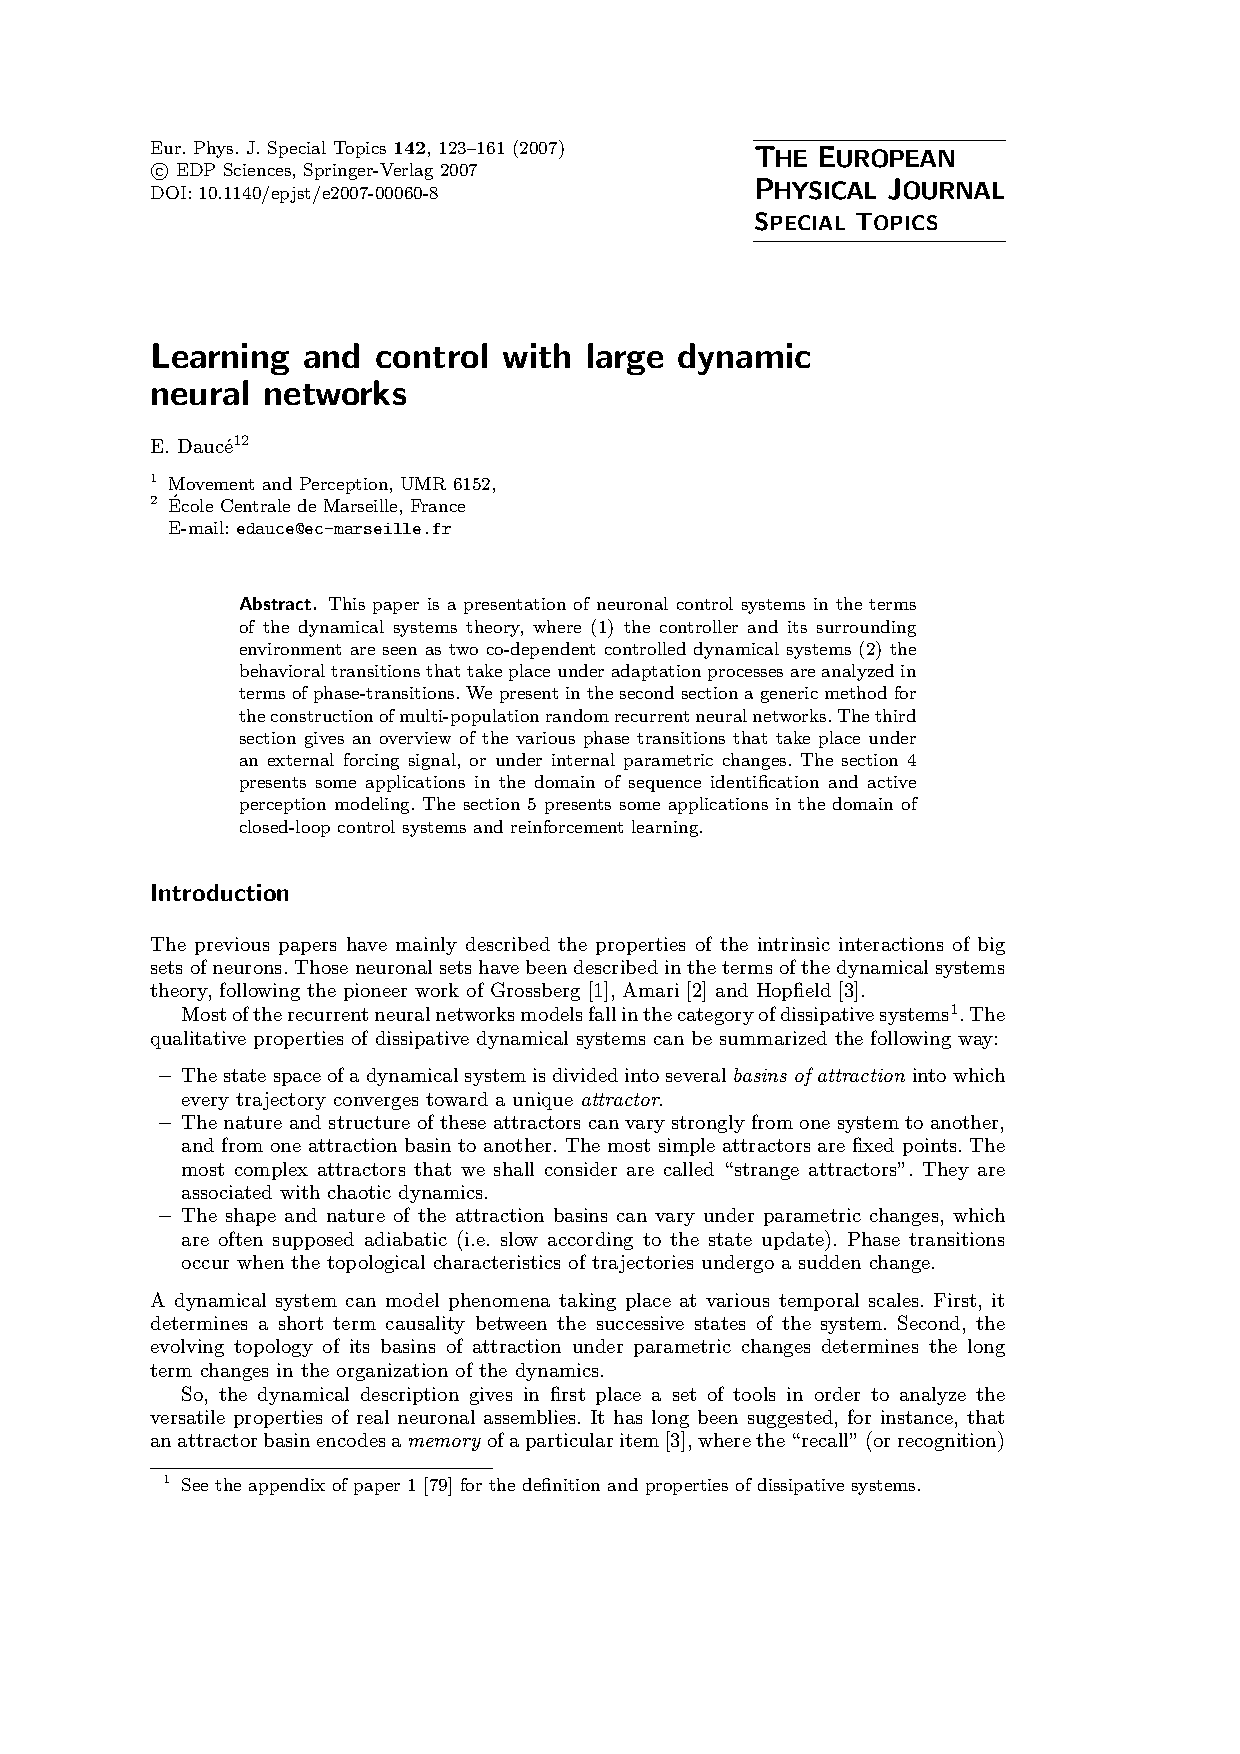
\includepdf[pages=1-10]{pdf/epj-st-2007.pdf}
%\end{minipage}
%}
% Histoires


%%%%%%%%%%%%%%%%%%%%%%%%%%%%%%%%%%%%%%%%%%%%%%%%%%%%%%%%%%%%%%%%%%%%%%%%%%%%%%%%%%%%%%%%%%%%%%%%%%%%%%%%%%%%%%%%%%%
%%%%%%%%%%%%%%%%%%%%%%%%%%%%%%%%%%%%%%%%%%%%%%%%%%%%%%%%%%%%%%%%%%%%%%%%%%%%%%%%%%%%%%%%%%%%%%%%%%%%%%%%%%%%%%%%%%%
%%%%%%%%%%%%%%%%%%%%%%%%%%%%%%%%%%%%%%%%%     4      %%%%%%%%%%%%%%%%%%%%%%%%%%%%%%%%%%%%%%%%%%%%%%%%%%%%%%%%%%%%%%
%%%%%%%%%%%%%%%%%%%%%%%%%%%%%%%%%%%%%%%%%%%%%%%%%%%%%%%%%%%%%%%%%%%%%%%%%%%%%%%%%%%%%%%%%%%%%%%%%%%%%%%%%%%%%%%%%%%
%%%%%%%%%%%%%%%%%%%%%%%%%%%%%%%%%%%%%%%%%%%%%%%%%%%%%%%%%%%%%%%%%%%%%%%%%%%%%%%%%%%%%%%%%%%%%%%%%%%%%%%%%%%%%%%%%%%

\section{Architectures de contrôle pour les neurosciences}

%%%%%%%%%%%%%%%%%%%%%%%%%%%%%%%%%%%%%%%%%%%%%%%%%%%%%%%%%%%%%%%%%%%%%%%%%%%%%%%%%%%%%%%%%%%%%%%%%%%%%%%%%%%%%%%%%%%

principe général : 
- comportement based
- mapping des architectures de contrôle sur le SNC

%%%%%%%%%%%%%%%%%%%%%%%%%%%%%%%%%%%%%%%%%%%%%%%%%%%%%%%%%%%%%%%%%%%%%%%%%%%%%%%%%%%%%%%%%%%%%%%%%%%%%%%%%%%%%%%%%%%
%%%%%%%%%%%%%%%%%%%%%%%%%%%%%%%%%%%%%%%%%     4.1      %%%%%%%%%%%%%%%%%%%%%%%%%%%%%%%%%%%%%%%%%%%%%%%%%%%%%%%%%%%%
%%%%%%%%%%%%%%%%%%%%%%%%%%%%%%%%%%%%%%%%%%%%%%%%%%%%%%%%%%%%%%%%%%%%%%%%%%%%%%%%%%%%%%%%%%%%%%%%%%%%%%%%%%%%%%%%%%%

\subsection{Modèles de l'orientation spatiale}

{\bf 2010}

- A. Mouraud : mecanisme integrateur. Dual drive. 


%%%%%%%%%%%%%%%%%%%%%%%%%%%%%%%%%%%%%%%%%%%%%%%%%%%%%%%%%%%%%%%%%%%%%%%%%%%%%%%%%%%%%%%%%%%%%%%%%%%%%%%%%%%%%%%%%%%
%%%%%%%%%%%%%%%%%%%%%%%%%%%%%%%%%%%%%%%%%     4.2      %%%%%%%%%%%%%%%%%%%%%%%%%%%%%%%%%%%%%%%%%%%%%%%%%%%%%%%%%%%%
%%%%%%%%%%%%%%%%%%%%%%%%%%%%%%%%%%%%%%%%%%%%%%%%%%%%%%%%%%%%%%%%%%%%%%%%%%%%%%%%%%%%%%%%%%%%%%%%%%%%%%%%%%%%%%%%%%%

\subsection{Modèles de l'orientation temporelle}

{\bf 2010}

- Gaurav : attention temporelle. Modele EM. 


{\bf 2011}

- scalar property

$\Rightarrow$ prior $\simeq$ ``\% up to now'' (subjective time)


%%%%%%%%%%%%%%%%%%%%%%%%%%%%%%%%%%%%%%%%%%%%%%%%%%%%%%%%%%%%%%%%%%%%%%%%%%%%%%%%%%%%%%%%%%%%%%%%%%%%%%%%%%%%%%%%%%%
%%%%%%%%%%%%%%%%%%%%%%%%%%%%%%%%%%%%%%%%%     4.3      %%%%%%%%%%%%%%%%%%%%%%%%%%%%%%%%%%%%%%%%%%%%%%%%%%%%%%%%%%%%
%%%%%%%%%%%%%%%%%%%%%%%%%%%%%%%%%%%%%%%%%%%%%%%%%%%%%%%%%%%%%%%%%%%%%%%%%%%%%%%%%%%%%%%%%%%%%%%%%%%%%%%%%%%%%%%%%%%

\subsection{Apprendre et oublier dans les environnements non-stationnaires}

{\bf 2011}

- Policy gradient dans les BCI. Reward adaptatif. Baseline optimale. 

{\bf 2013}

- Oddball problem / lien avec convolution networks et/ou ranking.

- Approche adaptative des BCI : label free logistic gradient descent avec accumulation d’évidence + subject-independent classifier.

- Hongliang : Passive Agressive + bandit feedback




%%%%%%%%%%%%%%%%%%%%%%%%%%%%%%%%%%%%%%%%%%%%%%%%%%%%%%%%%%%%%%%%%%%%%%%%%%%%%%%%%%%%%%%%%%%%%%%%%%%%%%%%%%%%%%%%%%%
%%%%%%%%%%%%%%%%%%%%%%%%%%%%%%%%%%%%%%%%%%%%%%%%%%%%%%%%%%%%%%%%%%%%%%%%%%%%%%%%%%%%%%%%%%%%%%%%%%%%%%%%%%%%%%%%%%%
%%%%%%%%%%%%%%%%%%%%%%%%%%%%%%%%%%%%%%%%%%%%%%%%%%%%%%%%%%%%%%%%%%%%%%%%%%%%%%%%%%%%%%%%%%%%%%%%%%%%%%%%%%%%%%%%%%%
%%%%%%%%%%%%%%%%%%%%%%%%%%%%%%%%%%%%%%%%%%%%%%%%%%%%%%%%%%%%%%%%%%%%%%%%%%%%%%%%%%%%%%%%%%%%%%%%%%%%%%%%%%%%%%%%%%%
%%%%%%%%%%%%%%%%%%%%%%%%%%%%%%%%%%%%%%%%%%%%%%%%%%%%%%%%%%%%%%%%%%%%%%%%%%%%%%%%%%%%%%%%%%%%%%%%%%%%%%%%%%%%%%%%%%%
%%%%%%%%%%%%%%%%%%%%%%%%%%%%%%%%%%%%%%%%%%%%%%%%%%%%%%%%%%%%%%%%%%%%%%%%%%%%%%%%%%%%%%%%%%%%%%%%%%%%%%%%%%%%%%%%%%%
\chapter{Projet scientifique}
%%%%%%%%%%%%%%%%%%%%%%%%%%%%%%%%%%%%%%%%%%%%%%%%%%%%%%%%%%%%%%%%%%%%%%%%%%%%%%%%%%%%%%%%%%%%%%%%%%%%%%%%%%%%%%%%%%%
%%%%%%%%%%%%%%%%%%%%%%%%%%%%%%%%%%%%%%%%%%%%%%%%%%%%%%%%%%%%%%%%%%%%%%%%%%%%%%%%%%%%%%%%%%%%%%%%%%%%%%%%%%%%%%%%%%%
%%%%%%%%%%%%%%%%%%%%%%%%%%%%%%%%%%%%%%%%%%%%%%%%%%%%%%%%%%%%%%%%%%%%%%%%%%%%%%%%%%%%%%%%%%%%%%%%%%%%%%%%%%%%%%%%%%%
%%%%%%%%%%%%%%%%%%%%%%%%%%%%%%%%%%%%%%%%%%%%%%%%%%%%%%%%%%%%%%%%%%%%%%%%%%%%%%%%%%%%%%%%%%%%%%%%%%%%%%%%%%%%%%%%%%%
%%%%%%%%%%%%%%%%%%%%%%%%%%%%%%%%%%%%%%%%%%%%%%%%%%%%%%%%%%%%%%%%%%%%%%%%%%%%%%%%%%%%%%%%%%%%%%%%%%%%%%%%%%%%%%%%%%%
%%%%%%%%%%%%%%%%%%%%%%%%%%%%%%%%%%%%%%%%%%%%%%%%%%%%%%%%%%%%%%%%%%%%%%%%%%%%%%%%%%%%%%%%%%%%%%%%%%%%%%%%%%%%%%%%%%%

{\bf 1999}

- Philo 1 : non-extensivité des sensations - analogie “zone aveugle”

{\bf 2000-2001}

- travail de biblio sur l’hippocampe. 

{\bf 2003-2004}

- Philo 2: pensée à l’échelle temporelle de nos actes

{\bf 2009}

- travail sur les structures sous-corticales : striatum/tectum/cervelet 

{\bf 2010}

- Premier modele (nu,theta)

En particulier : la notion d'expressivité du substrat est prometteuse. 

- Variables de contrôle. Equilibre dynamique. Homeostasie. Emploi et Couplage sans emploi. Répertoire (dictionnaire?) d'emplois. 

- Neurone hédoniste.
IDEE : DU POINT DE VUE DU NEURONE HEDONISTE, LES SPIKES EMIS DOIVENT AVOIR POUR CONSEQUENCE DE MIEUX SOUMETTRE LE NEURONE A DE NOUVELLES STIMULATIONS - PRIOR SUR L’EXPOSITION AUX STIMULATIONS FUTURES.




Perspectives :
\begin{itemize}
\item Substrat apprenant universel
\item Field computation. Patron (fenêtre) d’interaction anisotropique. La reponse n’est pas un vecteur ou un scalaire mais une distribution.
\item Regles de plasticité, information mutuelle et binding. Synchronie des systemes en interaction. Le binding au niveau des schémas d’interaction en miroir. Co-evolution. Mutual information (avec mutual emission et reception). Accrochage de phase. Emergence et non-sens. Independance : est “bindé” ce qui évolue ensemble (non indépendamment). Est “non bindé” ce qui évolue indépendamment. Lié aux DDL? 
$\Rightarrow$ Le substrat est le support de plusieurs processus indépendants. Par analogie au neural field, on peut avoir plusieurs “bulles” sur la carte.
\item idée de perméabilité / imperméabilité des echelles BOTTOM $\rightarrow$ UP. Les etats et les processus des echelles inferieures ne sont pas impactées par les phenomenes d’ordre superieur autrement que par les signaux et les tâches traitées à leur échelle. Exemple : une couche motrice est principalement en train de stabiliser des couplages, pas d’instituer (proclamer/décréter) un nouvel “emploi”. (pas de “downward causation”)
\end{itemize}

\chapter{Conclusion}

Les fondateurs des sciences cognitives ont placé très tôt la question de l'apprentissage  au coeur de leur problématique 
(qu'est-ce qu'une machine intelligente - cf. Turing)

Deux approches/réponses se dessinent dès l'origine :  
\begin{itemize}
 \item traitement symbolique
 \item traitement analogique
\end{itemize}
L'enjeu principal est celui d'un côté du traitement analogique et de l'autre le traitement symbolique. Du point de vue des sciences cognitives naissantes, c'est le traitement
symbolique qui gagne dans un premier temps.

Dans ces deux formalismes, la question de l'apprentissage a eu tendance à progressivement se marginaliser au profit (1) du traitement logique des symboles et de modèles
 descriptifs du langage (grammaires génératives) et (2) l'ingéniérie et la conception de systèmes d'asservissement de plus en plus complexes et/ou psychologie et constructivisme (Palo Alto)

A l'inverse, la question de l'apprentissage est restée présente dans le domaine des sciences de l'information et l'informatique naissante. 
La question de l'apprentissage  devient la question de construire des programmes (des automates) capables de se modifier, de s'amender pour mieux répondre aux sollicitations
de l'environnement. Cette question étant posée (comment modifier le programme sans intervention humaine), le formalisme des réseaux de neurones et du calcul distribué 
s'est révélé le plus apte à traiter la question --> le perceptron. 

\end{document}
